\documentclass{book}

\title{{\small Extracts from}\\ \vspace{12pt}{\Huge Aerial
    Sport}\\{\Large How and Why I Built the Pou-du-Ciel}}

\author{Henri Mignet\\
  {\small (translated by Jason R. Fruit)}}
\date{2019}

\usepackage[a5paper]{geometry} %% this makes a handbook
\usepackage{frcursive}
\usepackage[T1]{fontenc}
\usepackage{graphicx}
\usepackage{tikz}

%% Altered from a tex.stackoverflow.com answer to make smaller circles
\newcommand*\circled[1]{\tikz[baseline=(char.base)]{
    \node[shape=circle,draw,inner sep=1pt] (char) { #1};}}

\newcommand*\sectline{
  \vspace{5pt}
  \begin{center}
    \rule{0.5\linewidth}{\linethickness}
  \end{center}
  \vspace{5pt}
}

\begin{document}

\maketitle
\tableofcontents

\fontfamily{ppl}\selectfont

\chapter*{Translator's Note}

I have not presented Henri Mignet's little book in its entirety, but
\textit{ars longa, vita brevis}; I want to move on from translation to
build the little airplane about which I have read.  I must apologize
for this failing, however, because his writing is an absolute
pleasure, and his ideas are engaging and inspiring.

If you find errors of fact in my translation, please contact me at
\texttt{JasonFruit@gmail.com} with improvements, or submit a pull
request via \texttt{git} at
\texttt{https://github.com/JasonFruit/sport-de-lair}.  If you find
stylistic improvements that could be made, feel free to make your own
translation.  Better yet, go build an airplane.

\chapter*{1985}

The previous edition of this work was published in 1937.

It sold out quickly.  By the end of the war, it was almost impossible
to procure a copy.

Much time has passed.  Much has changed.  Some aeronautical disorder
has given way to a new order --- which is not necessarily an
improvement.

Henri Mignet, fleeing the memory of a terrible tragedy, hung his hat
in every corner of the world, leaving his faithful to preserve the
Flame.

During his absence, some amateurs, attracted to aeronautics by his
Pou-du-Ciel, relaunched the movement he had started, forming the
\textit{R\'eseau du Sport de l'Air}, the successor to the RAA.

Many productions saw the light of day --- especially classic aircraft,
these last sometimes with the financial encouragement of the state.

The results were so remarkable that these same amateurs at times
became artisans, and even industrialists!

In this manner was our current light aviation born.

When the Patron Saint returned home in 1958, he brought with him
wonderful memories and spiritual treasures.  But also, he brought back
notes for projects being carried out by his successors.

Henri Mignet is no longer with us.

\begin{samepage}
  
But here, thanks to some good friends, and thanks too to the
\textit{R\'eseau du Sport de l'Air}, just mended, barely completed, is

\center{\large \textbf{LE CHER BOUQUIN}}

\begin{flushright}
  Pierre MIGNET\\Les Pierri\`eres\\October 1985
\end{flushright}

\end{samepage}

\chapter{HOW I BUILT MY POU-DU-CIEL}

\begin{verse}
  { \fontfamily{frc}\selectfont If you can nail up a shipping
    crate,\\ You can build a Pou-du-Ciel\footnote{I hold this slogan
      as necessary criticism of my opponents. Is it a joke? --- No!
      It's a skillful camouflage\ldots I needed this propaganda,
      without which my book would have been dull, sad, turbid, and
      monotonous; without which I would not have started anything;
      without which 500 future airmen would not have built their
      airplanes; without which the public would never have seen at the
      \textit{15\textsuperscript{e} Salon de l'A\'eronautique 1936},
      two galleries of the \textit{Grand Palais} occupied by 31 light
      aircraft (Brochet, Sfan, Bassou, Voliand, B\'echeraud,
      Tr\'ebucien, Taupin, Cri-Cri, L\'eopoldoff, Mauboussin,
      Moustique), dominated by a squadron of 3 of the latest
      Pou-du-Ciel models!
      
      (As for building a solid packing box, it's harder than you
      think!)}.
    
}
\end{verse}


What is an aircraft?

\begin{itemize}
\item
  A body with tail-feathers, pulled forward by a propeller, securely
  suspended under a bearing surface that it pulls along.
\item
  A chain, the many links of which must all be equally solid. If only
  one link gives way, the system will cease flying.
\item
  A combination of simple elements that appear complicated.
\item
  An ordinary structure, of no precise adjustment, which still
  requires that everything should keep its shape.
\end{itemize}

\section{Material}

\begin{verse}
  The forest. A tree.\\
  Cut down. Sawn. Split. Dried.\\
  Carpenter - Band saw - Planer.
\end{verse}

A straight board, squared up, shining, veined with pink, supple,
stiff, light, fragrant. This material is no longer merely a
\emph{tree}.  Cut to length, bent, glued, nailed, sanded, varnished:
now here is a part of a whole, filling a void, a specific destiny,
occupying a particular place in the world, fulfilling its proper role.

It commands rapt attention: we look at it, we touch it, we evaluate
it, we care for it. It has \textit{personality}. It did not exist
heretofore; now it is born, it \textit{is}.

It has life, like a painting, a work of art. It will have adventures.
It will age, it will die --- in an attic, at the junk shop, or in an
accident --- like a being given life in a bed, in the hospital, or in
the railway --- like you, its creator.

Does it not spring from your blood? --- Bought ready-made, what would
you see in it?  A commodity, nothing more.  But in this, if it were
exchanged for money, marketed, sold, or given away, you would lose a
piece of yourself\ldots

You have no emotional attachment to a plaster-of-Paris statue, to a
car, stamped out by machines tended by bored employees. But you have
affection for what is lovingly carved by a craftsman, because he
placed his soul therein.

Having bought a tool, whatever object, I do not enter into its actual
possession, I do not become attached to it, except after
disassembling, improving, and reassembling it correctly, giving it a
state of completion that is incompatible with mass-production, where
the distracted hand of the worker refuses to honestly finish it.

Is there another piece of the airplane that is more attractive than
the propeller, the beautiful propeller with a slender curve that you
have so carefully sanded and varnished?  It is a symbol, it is a
sculpture in wood, personifying our object: the emblem of Aviation!

The material we craft is alive and sensitive, entitled to a
\textit{caress}.

What will be its destiny? Over what clouds, what valleys will it soar?
To what regions will I be carried, reclining on its cushions, belted
to its seat? --- It bears, latent, a full slate, a lifetime of
adventures.

From just a piece of wood it takes shape; its fate, still unknown to
me, is there, before me, under my hand, invisible, as I father it; I
am author of a life whose course I do not know, to which my body will
be bound in an intimacy sometimes joyous, sometimes hard and serious!

\begin{verse}
  A pretty story? --- A reality.\\
  Imagination? --- Real-life adventures!
\end{verse}

The material thus shaped \textit{lives}. It will live more fully under
the effect of the engine. It will age with use, it will ``grow up'';
the sides of the cabin will be weathered with oil, blackened by
exhaust, grass-stained\ldots the cabin soiled, worn, scuffed by shoes,
blackened at the back, pierced with now-useless holes, marks left by
past experiments\ldots Flight, adventures, patched up bruises --- this
packing box evinces the accumulated past. Not everyone has such a full
life! Have a look at some old crate at the airfield. Can't you feel
the charm, hear the stories that emanate from its decrepit frame?

\textbf{Respect.} --- So, a kind of friendship --- I almost said, love
--- makes you feel that the materials for this special construction
must be touched only with clean hands. Respect the material. Do not
brutalize it.  Wood is not only of the tree: it is a longeron, a
rib. Look at it closely; see if it is healthy.

Smoothness on the outside, detailed on the inside. Finish your pieces
well; round over the sharp corners, scrape away the spots.  Let the
viewers congratulate you on your work.

The amateur is like the sailor: He is a jack-of-all-trades,
universal. Overmuch mathematical baggage is not necessary to him. His
handyman skills are enough to salvage delicate situations. Above all,
he has a huge dose of ``common sense''. For this, there is no
school. With a little money and a lot of common sense, the amateur who
knows which way to turn a nut will succeed at this too.

\section{Humility}

The processes I outline here spring from my observations and the
outcome of an amateur's life work: they are made for amateurs.

I have intentionally adopted simple, rustic methods, to avoid
professional techniques which would scare off the amateur or
needlessly exhaust his time and patience.

Some will find our methods rudimentary --- "just do this, do that",
you will be told!  Avoid those people like the plague, and beware
anyone who believes they have some mystical secret!

I do not give you a choice of several models. In my previous edition,
I displayed my "Pou-du-Ciel" still quivering from its first ten hours
of flight. The same was exhibited at the 14\textsuperscript{e} salon
de l'A\'eronautique after 60 hours. It then had its feathers plucked
and was modified, transformed in search of progress. I have refined
the details, but the formula has remained the same. I have some 300
hours of flight in the Pou-du-Ciel. My latest model does not have much
over one that is 100\% from the book.

Life has forced industriousness on me.

The inadvertent advertising that my dear little book created among the
amateurs has raised in the general public a feeling of client\`ele,
setting for me certain conditions. The "Pou-du-Ciel" has excited
aviators and potential buyers. But they dream of performance, of
comfort; they want Aviation, the Pou-du-Ciel way. I've searched for it
--- I've found it --- but I can no longer be merely an amateur.

Will I, in this new book, describe to you not only the Pou 100\% by
the book, but also the Pou two-seat sedan? And then the Pou-B\'eb\'e
of less than 100 kilos? You, dear amateurs, you are good comrades; but
this little book is read also by less-good guys who will hurry up and
build a counterfeit Pou-du-Ciel, to profit from my labors, at the cost
of my little secrets and my reputation.

These new devices that I prepare and have already flown, what do they
do more than the Pou-of-the-Book? They fly faster, they climb
higher\ldots And then? They are made to be sold, but in the state you
are in, you, amateur builder, they would not give you more
satisfaction. New as they are, their construction by non-professionals
would risk danger. The Pou-of-the-Book has already had
misfortunes\ldots what would happen if I provided you with new models?
There are amateurs who would mix everything up, the government
agencies and trade organizations that protect the original formula
would be overwhelmed\ldots the opposition journalists would cover it
all in their sticky ink\ldots We would not see anything at all.

My honor is preserved by keeping to the Pou-of-the-Book. The friendly
help of the Ministry is not compromised, the troublemakers have no
reason to open their big mouths. Amateurs will soon be able to escape
the racetrack and Mignet the industrialist will not have completely to
shed his amateur's skin\footnote{The meaning of this passage,
  \textit{\guillemotleft Les amateurs pourront bient\^ot s'\'evader
    des tours de piste et Mignet l'industriel n'aura pas
    compl\`etement d\'epouill\'e la pelure de
    l'amateur.\guillemotright} may have been mangled in translation.}.

In doing this work, I tamed the beast as well as I could. The
Pou-du-Ciel of 1936 is almost a new aircraft, as it has improved its
flying qualities beyond its available power, as well as its comfort
and stability.

Do you want to fly like me?  Build according to the book, changing
nothing.

Don't worry your head.  Save your own innovations for later, after you
have 10 hours of flying.  You will judge your inventions from a very
different angle then --- believe me!

\section{Prudence}

All that flies must necessarily, be light --- granted.

One day when you repaint your craft, you will disassemble it. Out of
curiosity you put the pieces on the scales\ldots Five, six kilos too
much! You have made additions in recent flights!

From this day, the obsession grabs you, tenacious\ldots You have a
horror of weight. It becomes a mania! And you weigh, you streamline,
you lighten\ldots

Suddenly, reality hits: "It's crazy! my craft may have become fragile!
I'm losing my mind\ldots I do not know anymore\ldots"

And you are caught between hammer and anvil, between file and
wood. --- Too heavy? Too fragile? --- Dilemma!

Lightening a device does not just mean scraping away everything that
doesn't contribute to safety. It is not enough to turn a plywood board
into a colander, or to chamfer the corners of all square pieces: This
is called ``filing grams'' with a nail file.

The rational solution lies in a judicious, thoughtful plan, avoiding
complexity, reducing the number of important pieces. We then save the
kilos by tens. These few parts, then, can be reinforced: they only
weigh a few grams.

\section{Two-seaters}

You have not built yet. You admire aviation from a certain perspective.
You think: ``I will build a two-seater right away!''

Ah! Poor amateur! Poor imaginative! How many times have I been written
to about this damned two-seater! Everyone dreams about taking his
girlfriend up before he knows if he can rise above the daisies
alone!\ldots{}

Amateur aviation is a solitary sport, like horse-racing. The 40 kilo
jockey will always beat the fat one.

See the big touring two- or three-seaters prepare for a trip. It's
like a free balloon: Everyone scrimps on luggage: we have so quickly
accumulated 50 useless pounds! We can trade our parachutes for 30
liters of extra gas\ldots

Aviation is primarily a problem of weight. A two-seater? You'll never
fly in mono!

The two-seater will require 35 to 40hp, twice as much fuel, important
fees\ldots You won't find a suitable engine. You are stuck with a
single-seater\ldots you can't avoid it!  I do not want to hear any
more about amateur two-seaters. I will not answer!

\sectline

You will build a flying machine.

First, you will take off the ground. It's easy. --- Then you rise
above the fields, one or two meters. This is the big joy. --- Then you
go up.  Distant hills rising behind your familiar horizons. The top of
a tree goes under your wheels. The village steeple is lower than your
horizon\ldots The sky is under your butt!

Well \ldots what if your wings were to break at that moment?  Wouldn't
you feel a little thrill in your heart?

Me, I felt it. I do not feel it anymore. Not because I got used to the
danger, but because I superabundantly reinforced the points that
worried me. You will also avoid this unpleasant thrill if you follow
the directions of my book exactly.

Correspondents have sometimes asked me for full-size drawings, or
large scale blueprints, like they use in factories. What good would it
do?  Everything is specified already in the small ones! If you can't
read and understand them, you don't have the skill for this. Do not
begin building --- you will hurt yourself.

\section{Materials}

You will needlessly look for special ``Aeronautical'' raw materials
here. I chose a wood that is found in all lumber yards and carpenters'
shops: the fir tree of our furniture and our roofs. The dimensions
used are in agreement with its strength. If you find American wood,
spruce, Oregon pine, all the better. Similar weights, increased
strength --- do not change the dimensions. You would save a few
hectograms\ldots{} big deal!

For metal, I put myself in the shoes of the village amateur. I chose
mild steel sheet, because it pierces, files, and bends without special
precautions. I strongly reject the use of more or less hardened
aluminum in the vital fittings, \textit{e\.g\.} in the bracing of the
wings.

A single metal for the amateur: sheet metal; tubes; rods drawn or
threaded; bolts; all in mild steel from any hardware store.

The mild steel sheet joined to wood by small bolts will endure
vibrations and resonances indefinitely.

\textbf{\emph{Long live steel! Long live wood!}}

\section{Accessibility}

The Pou-du-Ciel is a simple design.

The most basic prudence suggests that you should entrust your life
only to a simple mechanism --- simple and verifiable.

A bolt a nut, a pin, when it is accessible, can be checked. It will
not shirk its duty. Hidden, the best-secured piece will eventually
come loose --- and your goose will be cooked.  We may find the
explanation, but it will be too late.

The entire mechanism of an aircraft must be visible, accessible,
verifiable, easily removable. Then, you will live. Otherwise, it will
kill you.

This is a law of Nature.

I did not cowl my engine; I placed all my controls externally; my
braces are at my fingertips. The fuselage is an empty box. Inspection
is possible.

\section{Regulation}

I do not know the future, and neither do you. Anything could happen,
even kindness from the government.

The \textit{Bureau Veritas} controls the ``Pou-du-Ciel''. The
\textit{Services du Minist\`ere} will make its decision. The book
currently serves them as a basis. If you have not followed my
instructions strictly, you may be refused

\begin{center}
  \textbf{ \large \emph{permission\footnote{M. Mignet says, ``the
        right to fly,'' but no-one can remove from you a right.  They
        may deny you permission, but \textit{you still have your
          rights!} --- Translator} to fly.}}
\end{center}

I urge the official inspector to examine your device (which will not
yet be covered, of course) to see that it is \emph{according to the
  latest requirements} for the correct installation of the braces, the
wing pivots, joins of the covering, choice of materials, and the wood
used: \textit{i\.e\.} no knots, straight grain, \textit{etc}.

Any permission to fly must be categorically refused to the stubborn
mule who chooses not to follow the book.

The inspection of the Pou-du-Ciel is too easy for a catastrophic
defect to go unnoticed, and its flight balance is so straightforward
that a close examination will cover the inspector's responsibility.

The fruit of long experience and 150 examples having flown is this:
\textbf{The Pou-du-Ciel does not break in the air}.

\section{Patent}

When an inventor has created a new trick, he makes its paternity
official by providing the Ministry of Commerce and Industry an exact
description and a careful explanation. If it's really a new trick,
this will allow the inventor to claim priority. Should a dishonest
industrialist or someone simply unaware of the prior art of the
patent, build and sell a realization of the trick without the
patentee's consent, the patentee has the right to oppose him a court
of law. Occasionally the inventor even wins\ldots

The amateur handyman, passionately interested in a new machine, does
not\footnote{In France, at least, this was apparently true.} have the
right to build it for personal use, even apart from any profit.

The ``Pou-du-Ciel'' is patented in France and abroad. No manufacturer
has the right to sell, without the authorization of the inventor,
parts having the character of the Pou formula. Builders and buyers can
be likewise prosecuted, sooner or later, when the inventor sees fit to
take care of it.

Unusually, I detail in this book the construction of the Pou-du-Ciel
for amateurs, and permit him to build one himself, with his own hands,
or using the suppliers whose addresses I indicate. If he complies with
these conditions, the amateur will not be pursued legally. He should
not look at these restrictions as some commercial scheme. ``My''
amateurs know me; the ``others'' can check with the suppliers. It's
only natural for one who is honest with others to continue working
with those who have worked to his benefit.

\section{The Author's Responsibility}

The Pou-du-Ciel cannot break in the air. This is meant with regard to
normal use as a vehicle. Whether going by car, bicycle, boat,
horseback, etc., there are two ways to take a trip: carefully, or
recklessly.  Human foolishness, when unleashed, respects neither age
nor fortune, nor race, nor any other limit. Each does as he pleases;
each pays the consequences.  If you are cautious, as I am, if, like
the sailors and airmen of certain companies, who rightly understand
the possibilities of their equipment, and you fly when the weather is
fair, you will never get hurt.

\textit{The risk is infinitely less than on the road.}

Under these conditions, I take the moral responsibility: In conscience
I know not to engage in folly. I flew. My machine is solid. You can do
the same. I think I have everything planned, everything arranged so
trouble will not occur.

Many clubs, seduced by the simplicity of primary gliders, wanted, from
motives of economy and sportsmanship, to build their machines
themselves.  Apparent simplicity. Who could have known before the fact
that such a very hollow airfoil would cause the wings to snap?  That
piano wire constituted an insufficient brace?

Many accidents happen, including the most ordinary: a glider's wings
can collapse in flight when the pilot, being towed by winch, pulls the
release handle too sharply.  Thus Ferrero was killed in Tunis, in a
primary glider, in November 1933 --- eight days before experiencing
his HM.8.  Who could imagine, to see it so well finished, so
beautifully curved, that such a perfect glider would spin in in a
flash\ldots?

It is incontestable, in France as much as in Germany, that, in gliding
clubs, \textbf{there are many accidents} and \textbf{there are many
  injuries}.

The particular design of the Pou-du-Ciel and its construction put it
in an totally different class. I know what I did. I know what it can
do. I leave it to the future to show that it is, \textit{of all
  current aircraft}, the least deadly.

But I will have no regrets, no sadness, no emotion at all if I learn
that you have hurt yourself by acting foolish. This no longer concerns
me.

\section{To Fly!}

But you are wise. Your personal ideas set aside, you say, ``Mignet
flies. I want to imitate him, and soon, fly better than him. To avoid
delay, I will copy his machine exactly, to place me on the same level
immediately. And then after\ldots look to yourself, good fellow!''

The obsession with Air, Space, Volume is as old as mankind. It is an
unlimited vista of imagination: everyone wishes to try his own ideas.

The possession of the atmosphere is the most beautiful of man's
conquests.  Already we have gone beyond Nature on several points. Yet
a few secrets to penetrate, and we will have won.

Air travel is the height of diversity. To go by air is the least
dangerous and the least expensive of all.  It is impossible to foresee
the consequences of this novelty on the social economy of the
nations\ldots Light aircraft will be the essential mode of transport
in the coming new society.  They are as powerful and diverse in their
mode of action as the medium in which they move, the vast Ocean whose
invisible waves flit over our heads.

We are truly on the threshold of the aerial age, and it belongs to the
amateurs, thanks to their universal quality as innovators.

\sectline

Overcoming gravity, moving through three dimensions\ldots What a
strange fascination, what a wonderful science!  A contest of
ingenuities, a rivalry of innovation\ldots A record is broken, the
satisfaction of a difficulty overcome. The rival wins? --- A thrill of
jealousy says in your ear: "Me too --- one day, I'll beat you!"

{
  \fontfamily{frc}\selectfont
  \begin{center}
    {\Large Voil\`a le Sport de l'Air!}
  \end{center}
}

Even the smallest accomplishment proves the man.  Each one shows his
value, each produces a spark. A sensational record, even around the
world nonstop, does not diminish the accomplishment of the beginner
who, his device just completed, flies for a mere two seconds.  It is
\textbf{he} who built it, \textbf{he} who flew it.  It is to him, his
capable hands, his eyes alight with joy, that the praise redounds!

{
  \fontfamily{frc}\selectfont
  \begin{center}
    {\huge Voil\`a le Sport de l'Air!}
  \end{center}
}

Your "cuckoo" is no longer a simple frame covered with canvas and
braced with wires. It is a latent power.

You will shine it, polish your brass turnbuckles\ldots you will caress
your big propeller, inhaling its odor of varnish\ldots You rub down
your engine with its deep fins, a thoroughbred of modern mechanics,
whose heart will beat at your command, suddenly animating the machine
with the personality that belongs to a \textit{living being} endowed
with character, which in turn your reflexes must obey. It is your
child --- and your master.

It is a machine companion that you defend as your own self,
passionately loved, far beyond a man's watch or his camera --- it is
an old adventuring comrade.

Empty dreams?  Vain ambitions?

You will have crazy fun! You will learn to manage an engine other than
by the throttle: carb jets, spark plugs, mixture, tachometer --- all
of it\ldots

And you will fly for real: Your engine, simple aid, will sustain you
under your shining wing. You will live \textbf{la Vie de l'Air}, take
into yourself the reactions of the atmosphere, deeply, to satiety.
Perhaps, meeting eagles in flight, you will try to soar as they do,
engine off --- will you learn to employ the currents of the
breeze?\ldots

A formidable future, of which you may, unaware, become a Pioneer\ldots

{
  \fontfamily{frc}\selectfont
  \begin{center}
    {\Huge Voil\`a le Sport de l'Air!}
  \end{center}
}

\sectline

\chapter{Construction}

\section{Supplies}

\textit{Obviously, M. Mignet's suppliers from the
  now-distant past are no longer in business.  They have been omitted
  except where the discussion may have current interest.  The list of
  materials, however, is still of use. --- Translator}

\enumerate{
\item{Okoum\'e plywood}
  
  6 panels 200cm$\times$100cm, thickness 3mm (30 tenths)\\
  7 panels 200cm$\times$100cm, thickness 1.5mm (15 tenths)

There is special plywood available, such as 1mm Okoum\'e and 0.7mm
Birch (which costs 60 francs per square meter!). The Pou-du-Ciel does
not require it.

  
\item{Stick softwood: Northern fir, Sweden, Oregon pine, etc ...)

  6 5m lengths $15\times60$mm, or 10 pieces 3m 20cm in length\\
  10 4m lengths $20\times20$mm\\
  50 3m lengths $6\times12$mm

\item{Fabric and dope}

  Only approved Aviation supplies will do, not the cheaper, flimsier fabric.

  100m 40mm pinked tape\\
  30m\textsuperscript{2} standard fabric\\
  20L standard dope

  If you can afford it, get 40m\textsuperscript{2} fabric and 30L
  dope.

\item{Wheels}

  A good size is $450\times100$.

  The Lambert brothers have built a wheel in stamped and welded steel
  plate with bronze rim, for a 40mm axle, weighing 1kg 600. Equipped
  with Dunlop tires, it weighs 3kg 700.

  By agreement with me, these same Lambert brothers, who were
  practicing as amateurs at the time (1936) of the old HM.8 and the
  Pou-du-Ciel, have produced parts and fittings specially adapted to
  the Pou-of-the-Book. Ask them for a price. Whoever has not worked
  metal before will do better to buy his hardware. It will of course
  be more expensive, but faster and safer.\\
  \\
  \textbf{N.B.} --- I do not authorize any other person to sell spare
  parts, special fittings for the Pou-du-Ciel. The Lambert Brothers
  manufacture them under my control, and they give satisfaction. \textit{I
  receive no commission for it.} I warn the amateur against several
  counterfeiters (who will be pursued one day or another) and sell
  scrap iron shamelessly shaped, denatured: they are criminal thieves.

\item{Hardware}

  Seamless drawn steel tubes:

  4m $13\times16$\\
  4m $16\times18$\\
  2m $16\times20$\\
  2m $17\times20$\\
  2m $21\times24$\\
  50cm $24\times27$\\
  1m 20cm $31\times35$\\
  1m 20cm $36\times40$\\
  20cm $40\times44$\\
  \\
  Also, at your option, the drawbar: 1m 80cm $31\times35$.

  Mild steel plate:

  $30\times80$, 20 tenths.\\
  Other thicknesses (15, 10, 6 tenths) purchased as needed.

  Drawn mild steel rod: 2m each 4, 6, 8, and 10mm\\
  Threaded mild steel rod: 3m each 4, 5, and 10mm

  Steel bolts, with their nuts:

  50 $5\times40$\\
  30 $5\times 60$\\
  20 $6\times40$

  Have a good supply of hex nuts\ldots You won't lose by this ---
  because you will lose a lot of these!

  200 4mm\\
  200 5mm\\
  20 10mm lock nuts

  Extra flexible steel cable:

  10 meters in 5mm. for bracing; also 20 thimbles and 20 end fittings
  with 2 bolts.\\
  20 meters 2.4mm for controls; also 20 thimbles and 20 end fittings
  with 1 bolt

  \textbf{No galvanized cable, please.  Forget economy --- your life
    is at stake here!}

  Aluminum:

  1m\textsuperscript{2} 6/10 (rollovers, trim, etc.)\\
  2m 3mm aluminum wire (rivets, floats, etc.)

  Nails, steel, flat head:

  100g $1\times25$\\
  100g $1\times20$\\
  400g $1\times15$\\
  600g $0.7\times8$\\
  200g brass, 8 mm.

\item{Bungee}

  5m 12mm; it should start to stretch at about 38 pounds.

\item{Celluloid (windshield, windows, etc)}

  One sheet 1m20cm$\times$0.60$\times$1mm weighing 1kg.

\item{Glue}

  \textit{Of course we should no longer use casein glue! --- Translator}

  2kg Certus brand cold casein glue, powdered, in tins

\item{Tubes and light metals}

  Aluminum tubes, all thicknesses, all sizes, from $3.5\times4$mm\\
  Tubes de brass and copper (pitot and static tubes, fuel lines, etc.)\\
  
  Duralumin:

  20 tenths sheet, $50\times50\times1kg400$\\
  Tubes of all sorts, in T, L, U, etc. sections

  $21\times25.1$m $=$ 0kg 100}\\
  $17\times21.1$m $=$ 0kg 275\\
  $6\times8.1$m $=$ 0kg 75

  Expensive metal, and not suited for amateur use in vital parts of
  the machine.

\item{Fuselages, wings, rudders\ldots}

  The sale of these pieces ready-made, either whole or in parts,
  \textit{e.g.} spars, ribs, is unauthorized, except insofar as the
  advertisement carries the words "under the control of
  H. Mignet". Anyone unable to build the wood part of the
  "Pou-du-Ciel" is unworthy of the name, "Amateur" --- \textit{Ugh!}

\textit{(M. Mignet offers additional suggestions: a supplier for
  aeronautical maps and a subscription to the amateur aviation journal
  \guillemotleft Les Ailes\guillemotright.  The translator recommends membership in the
  Experimental Aviation Association (EAA) and subscription to its
  publication, Sport Aviation, as the best modern-day substitute for
  \guillemotleft Les Ailes\guillemotright. --- Translator)}

}

\chapter{To Work}

The amateur is an \textit{enthusiast}, an artist who obeys his
impulses.

The amateur wishes to grant himself wings. He would stick feathers on
the egg before the chick hatches to speed him along\ldots He will
start with the wings!

No!  I will subvert this logical order.

\sectline

We begin with the fuselage!

\section{Fuselage}

The fuselage is built like a crate. But since the plywood cannot be
nailed to itself, a pine member is fastened at the corners, as an
intermediary which receives the nails, which clamp the faces as they
are glued. In this way, the plywood faces are joined together not by
nails, which is flimsy, but by plenty of glue, which is like welding
the wood. When we say, "nail these", glue is implied, wherever wood
touches wood.  I saw wing ribs without glue, the tips of whose nails
too long, so they were folded back on the sticks they had pierced! I
also saw a fuselage whose nails, driven from inside the pine members,
barely penetrated the 3mm plywood.  No, dear child\ldots\ the head of
the nail must be on the plywood side to clamp it to the member!

\begin{figure}
  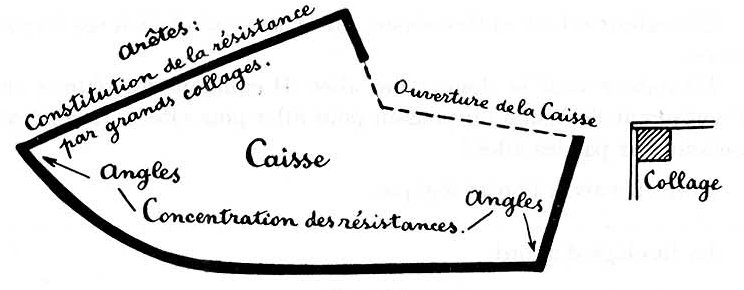
\includegraphics[width=\linewidth]{fig-15.jpg}
  \caption{The members concentrate the strength of the plywood}
  \label{fig:fifteen}
\end{figure}

The pine members concentrate the strength of the plywood, allowing
fittings to be attached to the corners of the box where the plywood
alone would have only a weak local resistance
(\textit{Fig. \ref{fig:fifteen}}). These corners are extremely strong nodes which
will form hard points for fittings.

The longerons behind the cabin extend its solidity to the rear, and
form an extremely rugged triangulated pyramidal structure.

At the risk of being a bit overweight, the fuselage is built entirely
of 3mm ply.  It will retain its strength.

\textit{(M. Mignet gives details about preparation of casein glue,
  which is no longer in use. --- Translator)}

\sectline

Before using it, examine the wood; it must be healthy.  No greenish
tinge suggesting the effects of worms; when planed, it should smell of
resin. The shavings, twisted like string, should resist traction.

Each member, carefully selected, is held in the vise by one end and
twisted along its length.  It must not break or crack.

Inspect it minutely: it must have straight or only slightly oblique
grain, without knots, splits, or shakes.

\subsection{Fuselage sides}

On a piece of 3mm plywood, lay out the first side according to the
dimensions in Figure \ref{fig:sixteen}.  The direction of the grain is
indicated by the arrows \textsl{f}.  Proceed according to the numbered
steps: \circled{1}, \circled{2}, \circled{3}, etc.

\begin{figure}
  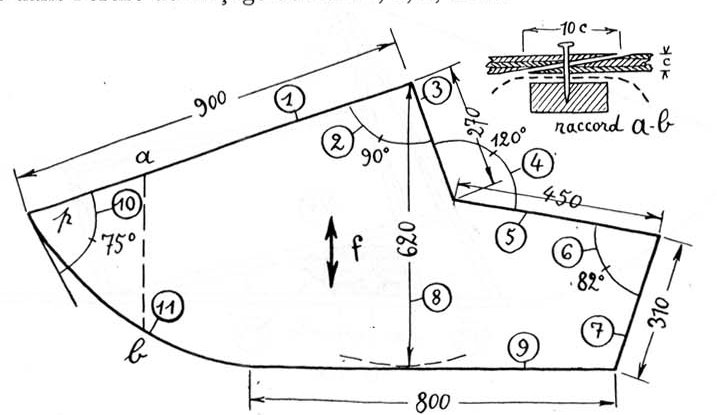
\includegraphics[width=\linewidth]{fig-16.jpg}
  \caption{Outline of fuselage side}
  \label{fig:sixteen}
\end{figure}

The dimensions are given in millimeters.  Determine the angles using a
protractor.

Cut two sides the same with a fine-bladed handsaw.

If the plywood is too small in the correct grain direction, choose a
point \textsl{p} on the segment \textsl{a---b} at which to make a
glued scarf joint.  Temporarily nail through the scarf joint into a
wooden piece covered with newsprint, which can be removed when dry.

A longeron $20\times20$, 2700\footnote{Both here and in the figure
  M. Mignet mistakes himself and writes 2800; the measurement in
  fig. \ref{fig:seventeen} is incorrect.} mm (2m 70cm) is glued and
nailed as at \circled{12}, fig. \ref{fig:seventeen}.  It extends
beyond the end of the side by 1900 mm.

\begin{figure}
  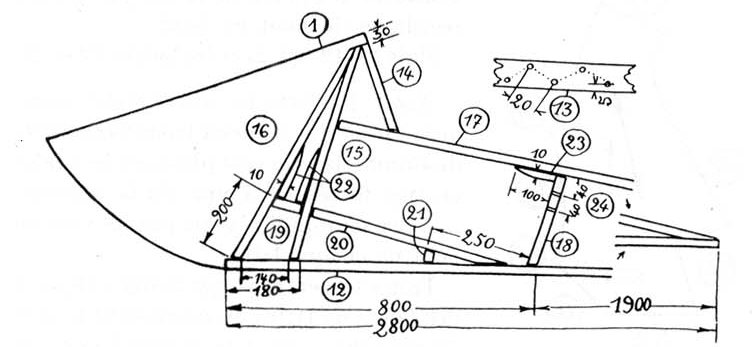
\includegraphics[width=\linewidth]{fig-17.jpg}
  \caption{Layout of longerons and members, fuselage side}
  \label{fig:seventeen}
\end{figure}

To glue, spread the glue on the first 800mm of the longeron, so there
are no bare spots.  A nail at each end will steady it while you nail
in a zigzag pattern every 20mm or so, as seen at \circled{13} in fig.
\ref{fig:seventeen}.  After nailing, the glue will be squeezed out
along the entire joint.  Plane it away when dry.

Continue fastening $20\times20$ members \circled{14}, \circled{15},
and \circled{16}, ending 30mm shy of edge \circled{1}.

Then put in place longeron \circled{17,} which runs from member
\circled{15} to end in a bevel against longeron \circled{12}, which is
straight from end to end.

Then \circled{18}, \circled{19}, \circled{20}, \circled{21}, and
blocks \circled{22} and \circled{23}.

\textbf{N.B.} Member \circled{18}, \textit{before it can be fitted},
must be drilled with two holes \circled{24} 40mm apart.  These are for
the 5mm threaded rods holding the safety belt.

Be careful to leave no gaps at the ends of the various members.

\begin{figure}
  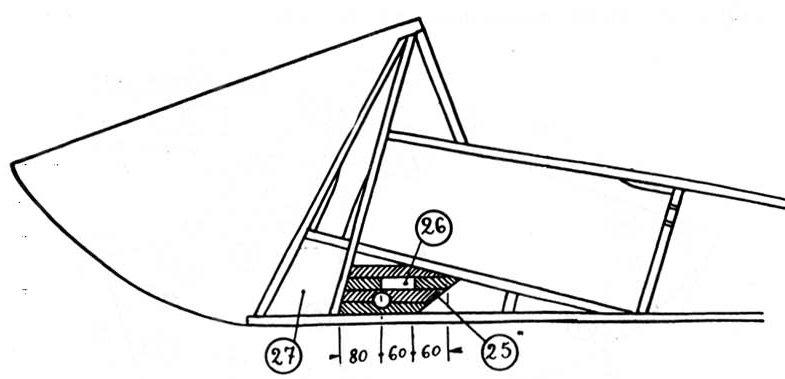
\includegraphics[width=\linewidth]{fig-18.jpg}
  \caption{Openings at bottom of cockpit}
  \label{fig:eighteen}
\end{figure}

Make the blocking \circled{25} in fig. \ref{fig:eighteen} with pieces
of slats, leaving the gap {26} which measures $20\times60$. With the
tip of a knife, remove the plywood over this void; the pulley of the
rudder cable will be placed there later.  Also remove the plywood
covering the quadrilateral \circled{27}, through which the axle will
pass.

Cover that assembly with plate \circled{28}, fig. \ref{fig:nineteen},
made of 3mm plywood, of which side \circled{1} is 150mm long.

\begin{center}
  \begin{figure}
    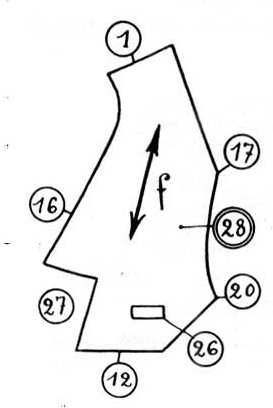
\includegraphics[width=0.5\linewidth]{fig-19.jpg}
    \caption{Plate inside front of cockpit}
    \label{fig:nineteen}
  \end{figure}
\end{center}

Prepare the second side, \textit{exactly like} the first, but
reversed; \textit{i.e.} with the longerons, members, etc. on what will
be its inside.

I must emphasize: wherever wood touches wood, you must glue and nail.

\begin{figure}
  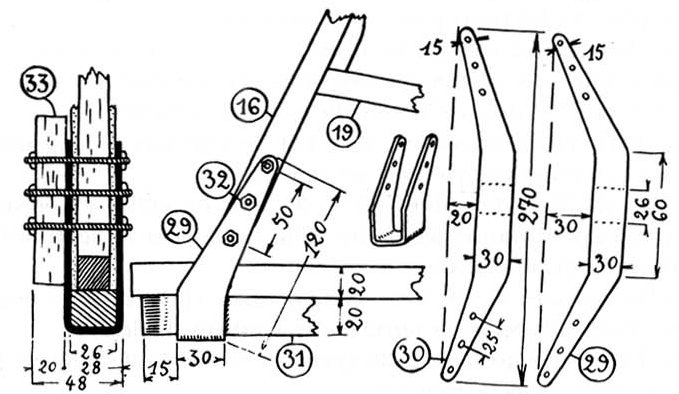
\includegraphics[width=\linewidth]{fig-20.jpg}
  \caption{Landing gear reinforcement}
  \label{fig:twenty}
\end{figure}

In a sheet of 1mm soft steel, cut two strips \circled{29} and
\circled{30}, which, when bent, will be held in place by gluing under
the lower ends of members 15 and 16 a pad, \circled{31}
(fig. \ref{fig:twenty}) of hardwood --- walnut, oak, beech, etc. ---
$20\times26\times230$.  Only drill one side of these fittings for now.
The other side will be drilled later when it is bound or clamped in
place.

The bolts \circled{32} of $5\times60$ threaded rod will further secure
the flanges \circled{33} of 20x20, which will be inside the fuselage.

\begin{figure}
  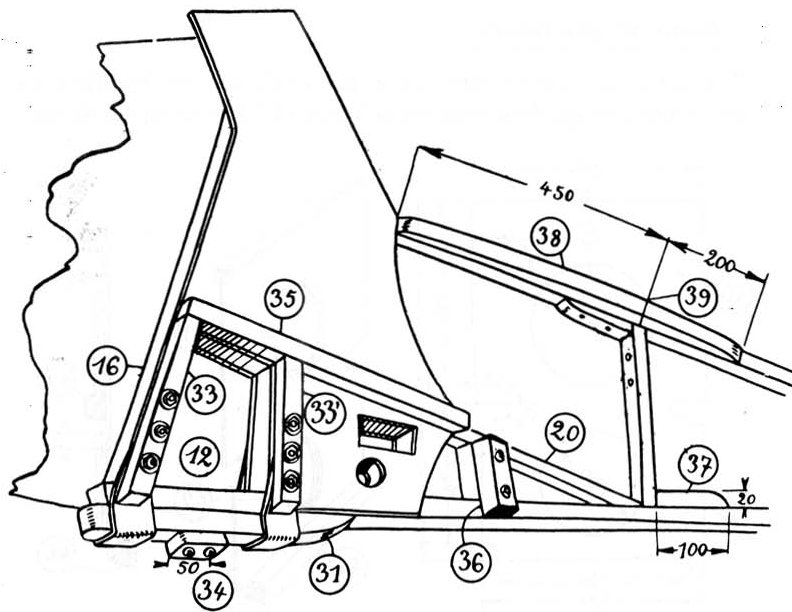
\includegraphics[width=\linewidth]{fig-21.jpg}
  \caption{The completed assembly around the axle}
  \label{fig:twentyone}
\end{figure}

Figure \ref{fig:twentyone} gives the overall appearance of the
finished assembly.

The pad and the flanges reinforce the longeron \circled{12} when the
axle strikes it in rough usage.

A hardwood block \circled{34} $10\times26\times50$ is glued and
screwed onto the pad at equal distance from the flanges. It will
prevent the bungee cord that secures the axle from slipping.

Glue on the wedges \circled{35}, \circled{36}, and \circled{37} ---
the latter made of hardwood --- to which the wing brace fittings will
later be bolted.

The reinforcing member \circled{38} is $20\times20$ at point
\circled{39} and thins gradually toward its ends.

\subsection{Joining the sides}

The two sides will be joined by the pilot's seat back \circled{40}, of
3mm plywood as in fig. \ref{fig:twentytwo}.  Holes \circled{41} and
\circled{42} are reinforced with plywood rings, and provide access to
the luggage compartments.

\begin{figure}
  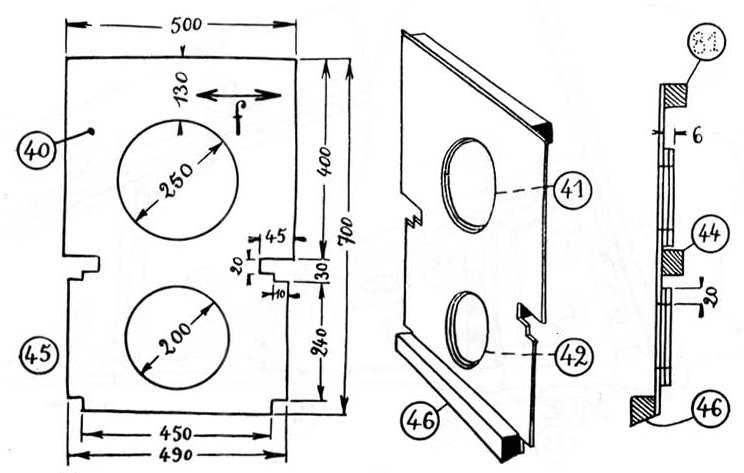
\includegraphics[width=\linewidth]{fig-22.jpg}
  \caption{Pilot's seat back}
  \label{fig:twentytwo}
\end{figure}

The holes and rings can easily be cut with a carpenter's compass with
one branch sharpened to a cutting blade.

On the panel \circled{40} place only the bar \circled{44},
$20\times20\times410$, and nail the sides \circled{45} in front of
member \circled{18}.  Then add cross-member \circled{46}, beveled to
be flush with the underside of longeron \circled{12}.

The front flanges \circled{33} are now joined by the panel
\circled{47} (fig. \ref{fig:twentyfour}, cut so that its cross member
\circled{48} fits on the shim \circled{35}, and its crosspiece
\circled{49} at the bottom of the tabs \circled{33} so that cross
members and flanges are flush with the longerons \circled{12}.  The
height of the panel \circled{47} will be determined in place.  Do not
forget that the hole \circled{50} is reinforced with a ring.  File
away what could interfere with the flanges \circled{29}.

\begin{figure}
  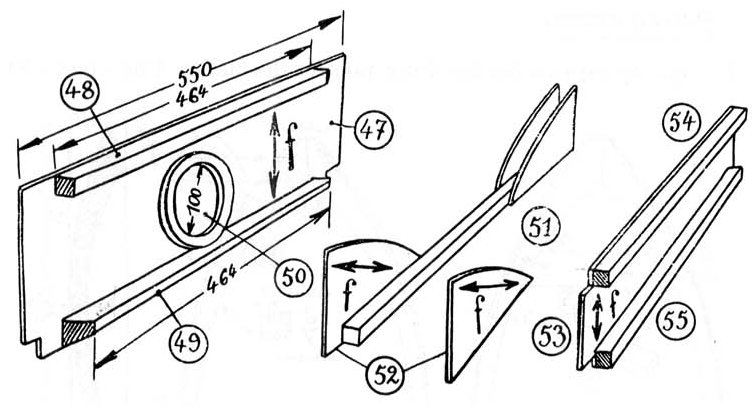
\includegraphics[width=\linewidth]{fig-24.jpg}
  \caption{Front panel joining sides}
  \label{fig:twentyfour}
\end{figure}

The rear flanges \circled{33} are joined at their lower part by a
member \circled{51} and double gussets \circled{52}.

The same goes for the flanges \circled{36}, joined by sheet
\circled{53} with members \circled{54} and \circled{55}.

The members \circled{46}, \circled{20}, \circled{35}, \circled{48} and
\circled{54} are all on the same plane, and support the seat-bottom
\circled{56}, which is seen from below in fig. \ref{fig:twentyfive}.
Determine its form in place with cardboard, so as not to waste plywood
unnecessarily. This panel is only secured by $12\times15$mm
round-headed wood screws. It is doubled, to a thickness of 6 mm and
glued under weights. Nailing would be useless.

\begin{figure}
  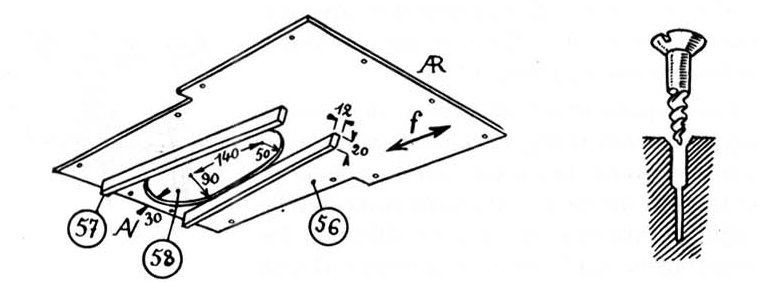
\includegraphics[width=\linewidth]{fig-25.jpg}
  \caption{Seat bottom from below}
  \label{fig:twentyfive}
\end{figure}

Two members \circled{57} stiffen the seat bottom between the
cross-members \circled{48} and \circled{54}, and the edges of the
central hole \circled{58} through which the control stick will pass.
At each end of the members, put in place a wood screw with a washer.

\textbf{Screws}: Before inserting a wood screw, drill a pilot hole
two-thirds the diameter of the solid metal part of the screw.  Rub the
threads with beeswax.

\sectline

\subsection{Front point}

The two ends of the flanks are brought together by a ``lyre''
\circled{50} cut with a saw from a 20mm hardwood plank
(fig. \ref{fig:twentyseven}).

\begin{figure}
  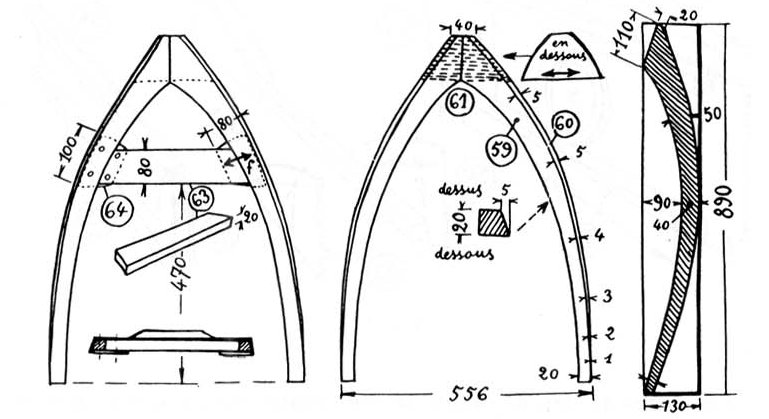
\includegraphics[width=\linewidth]{fig-27.jpg}
  \caption{The ``lyre''}
  \label{fig:twentyseven}
\end{figure}

Because of its incline relative to the fuselage, it will be necessary
to bevel its outside faces \circled{60}, to decrease the upper face
according to the progressive dimensions indicated: 0, 1, 3, 5, 5,
5. The branches will be separated by 556mm by adjustment of the joint
\circled{61}, which is reinforced below by the triangle of plywood
\circled{62}.  It is also stabilized in the middle by a board
\circled{63} of 20mm hardwood closely fitted and strengthened below by
6mm gussets \circled{64}. All this is to be well glued.. This board
will be reinforced by bolted fittings, and will support the engine.

Bevels, adjustments, and fitting should be begun with the plane and
finished with a large half-round bastard file --- for metal, not wood.
It should be bought and kept like new, used only for wood.  It is
preferable to a wood rasp, which tears out the grain, and after the
glue dries, it will munch away at the wood as well as the wood rasp,
even if there are nails --- which would ruin the rasp or the plane
immediately.

Put the two branches of the lyre together between the plywood sides
\circled{1} and the plywood panels \circled{28}
\textit{(fig. \ref{fig:twentyeight})}.  Nail so that the two sides
\circled{65} meet slightly past point \circled{66}.  Nail the plywood
all along the branches, about every centimeter.

\begin{figure}
  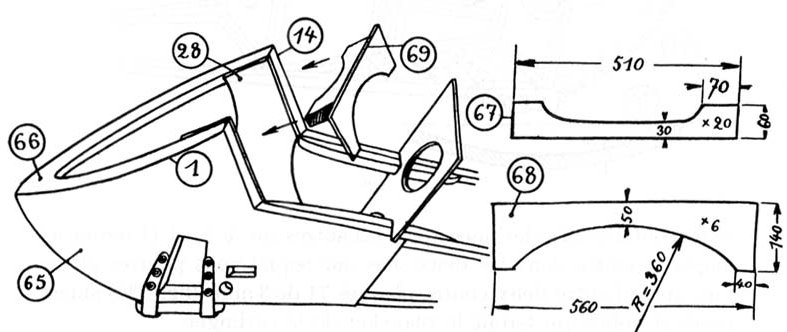
\includegraphics[width=\linewidth]{fig-28.jpg}
  \caption{Fastening the ``lyre'' in place}
  \label{fig:twentyeight}
\end{figure}

Cut off the excess of the branches of the lyre and plane away the side
material \circled{1} that extends above the lyre; for that purpose,
the sides were drawn out in Figure \ref{fig:eighteen} with 30 mm
instead of 20 mm.

From a 20mm hardwood board, cut out \circled{67} and nail under the
panel \circled{68}, 6mm thick, as seen at \circled{69}.  This will
connect the two branches of the lyre and the rim of the cockpit side
\circled{14}.

\subsection{Planking}

Turn your shipping crate upside down.

\begin{figure}
  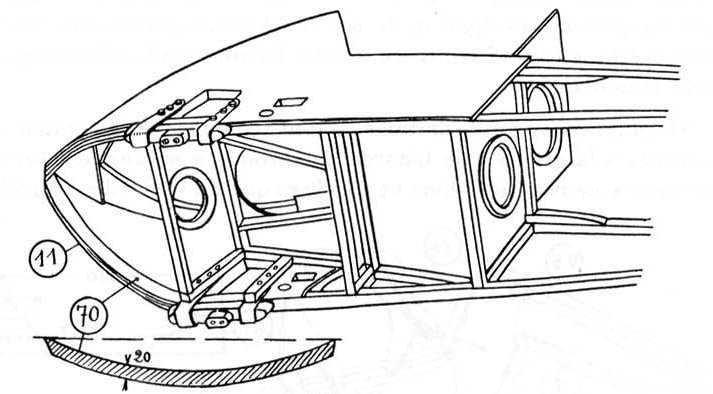
\includegraphics[width=\linewidth]{fig-29.jpg}
  \caption{Flanges to support cabin floor}
  \label{fig:twentynine}
\end{figure}

Cut out a strip \circled{70} \textit{(fig. \ref{fig:twentynine})},
25mm wide and fitted to the edge \circled{11}.  Copy it 14 times in
3mm plywood.  Seven thicknesses glued one after another inside each
side \circled{11} form a flange curved in both directions, on which
you can nail one after the other two 3mm plywood pieces \circled{71}
\textit{(fig. \ref{fig:thirty})}, layered and glued, which will serve
as the cabin floor.

\begin{figure}
  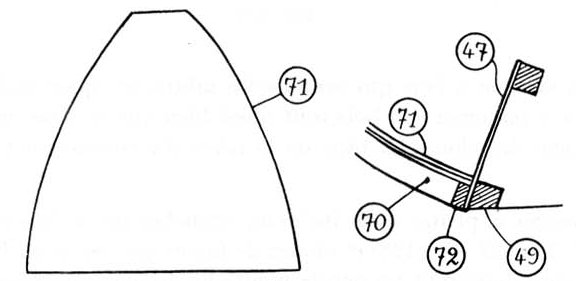
\includegraphics[width=\linewidth]{fig-30.jpg}
  \caption{Fitting the cabin floor}
  \label{fig:thirty}
\end{figure}

The floor is supported by a cross-member \circled{72},
$10\times20\times504$, fastened in front of panel \circled{47}.

With the file, align the lower faces of the flanges \circled{70}, so a
3mm plywood piece like a curved triangle will have good contact
everywhere from the point to the cross-member \circled{72}.  This
forms part of the bottom skin of the fuselage.

Now cover the lyre back to panel \circled{68} with 3mm plywood.

I am sure you have, by this point, sat in \textit{your cabin} already.
Am I right?

\begin{figure}
  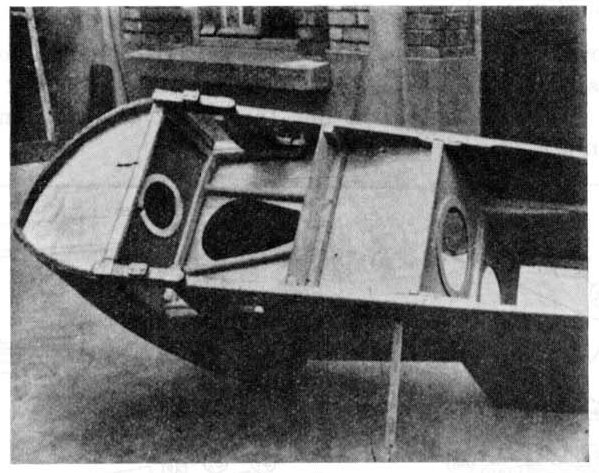
\includegraphics[width=\linewidth]{fig-31.jpg}
  \caption{The underside of a fuselage before applying the bottom skin
    in front}
  \label{fig:thirtyone}
\end{figure}

\begin{figure}
  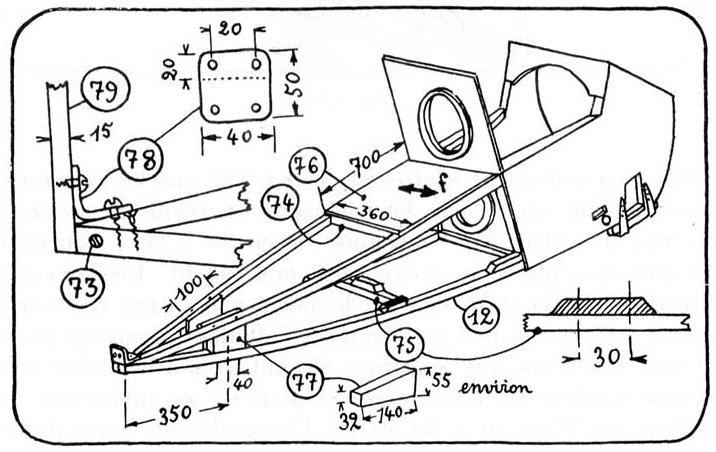
\includegraphics[width=\linewidth]{fig-32.jpg}
  \caption{Rear point}
  \label{fig:thirtytwo}
\end{figure}

\subsection{Rear point}

Join longerons \circled{12} and \circled{17} in a point
\textit{(fig. \ref{fig:thirtytwo})} with a wood screw \circled{73}
$4\times40$ with a countersunk head, making sure to insert members
\circled{74} and \circled{75} 700mm from the seat back.  Put in place
the luggage-box floor \circled{76} of 3mm stock, and two hardwood
wedges \circled{77} fastened with 2 $4\times40$ round-headed screws
spaced 40mm apart, reinforced internally with pieces of 3mm plywood
with the grain vertical.

Cut out two fittings \circled{78} in 1mm steel that will be folded
into angles.  One will be used to attach the hardwood tailpost
\circled{79}, $15\times40\times450$, to the rear point, using
$4\times15$ round-headed screws.  (This is a provisional attachment
pending completion of the final sides.)

\begin{figure}
  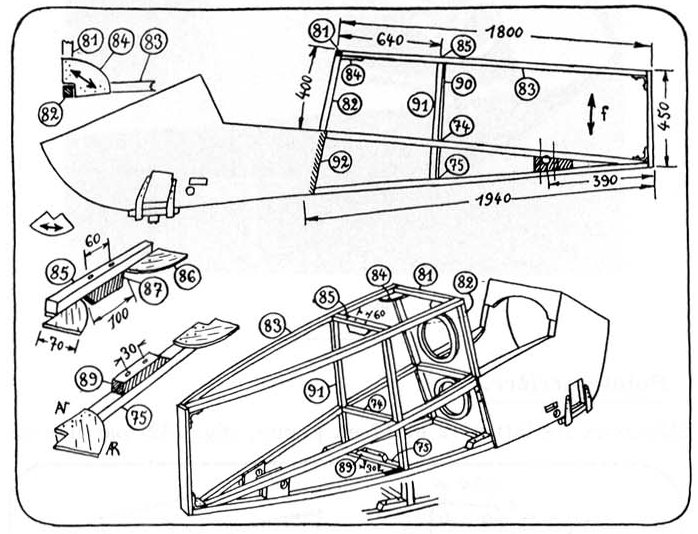
\includegraphics[width=\linewidth]{fig-33.jpg}
  \caption{Fuselage superstructure}
  \label{fig:thirtythree}
\end{figure}

Put in place the vertical and horizontal members \circled{81},
\circled{82}, fig. \ref{fig:thirtythree}, followed by the longerons
\circled{83} fixed to \circled{81} on the front by two gussets
\circled{84}.  The longerons are joined at the rear by a screw, and
held apart by the spacer \circled{85} (nailed with gussets) placed
about 640mm back from \circled{81}.  The members \circled{85},
\circled{74}, and \circled{75} are in the same plane, which, like the
tailpost, is almost vertical when the fuselage is placed on the
ground.  The longerons \circled{83} are affixed to the tailpost by the
second angled fitting \circled{78}.

The spacer \circled{85} has suspended in its middle a piece of
hardwood \circled{87}, $20\times20\times100$.  The assembly should
have two 6mm holes drilled through it, 60mm apart.  Similarly, spacer
\circled{75} bears a part \circled{89} with 2 6mm holes drilled
30mm\footnote{The text says 60mm, the diagram shows 30mm in two
  places; the text is probably in error.} apart.

While doing all this, make sure that the tailpost is aligned to the
cabin. Plane it down so that it follows the lines of the fuselage.

Put in place the bulkhead \circled{90} on members \circled{91} by
fastening it behind \circled{74}, \circled{75}, and \circled{85}.

Bevel the plywood sides with a file at \circled{92} so that you can
glue to them the rear sides, which will also be beveled, without
creating a bulge.  (That is, prepare a scarf joint.)

With the help of a few nails, apply a 3mm sheet of plywood to each
side.  Trace the required shape.  Cut it out and nail with plenty of
glue.  When nailing the second panel, make sure the tailpost is still
straight.  After it dries, clean up the edges with a plane or file.
At this point you have what is seen in fig. \ref{fig:thirtyfour}.

\begin{figure}
  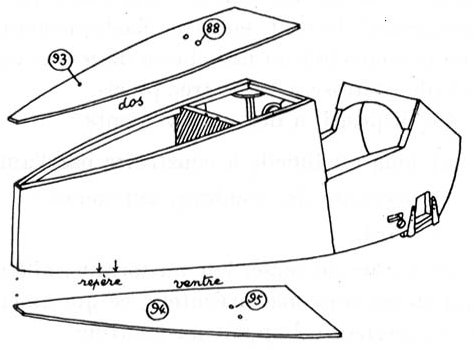
\includegraphics[width=\linewidth]{fig-34.jpg}
  \caption{Fitting the rear skins}
  \label{fig:thirtyfour}
\end{figure}

You can close the box with the lid \circled{93}, drilled with a 7mm
hole \circled{88}.  Remove the screws from the rear blocks
\circled{77} and precisely mark their position on the sides.  Then
install the bottom \circled{94} of the box, drilled with holes
\circled{95}, up against the seat.

Prepare the 3mm plate which will form the bottom between cross-members
\circled{46} and \circled{49}, but put it in place later.

The fuselage is complete.  You have built it in 4 days.  It weighs but
18 kilograms.  By skinning the back and bottoms with thinner plywood,
by shaving some members in excessively strong spots, the weight might
have been reduced by a kilogram.  Reinforcements and shims would have
had to be added, and even so, the plywood would soon warp.  A clumsy
move, a pebble, a branch of a tree, a wire dragging on the ground,
would have wrecked it.  Our machine is not a window display; it is to
be used.

\section{Landing Gear}

\subsection{Tailskid}

In the first edition, I had shown the rudder and twin biconvex wheel
as a solid assembly whose bearing axis was the rudder control, all as
a block, elastically attached to the fuselage.  The pilot could
maintain control both at flight speeds and taxiing at low speed.  It
was very precise.

This device had its disadvantages, however:

\enumerate{

\item{It was difficult and time-consuming for amateur construction}
\item{It required welding}
\item{It is heavy}
\item{It carried the risk of breaking on rocky ground, or if the welds
  were poor, which could cause a catastrophe if the rudder became
  uncontrollable}
\item{It was too easy to steer on the ground for learning}
\item{It dragged badly on landing}
}

In this edition, I abandon that system, and substitute the old
uncoupled rudder control and the well-known tail skid used on the
HM.8, which we amateurs have used and perfected.

\sectline

The trailing joint of the longerons \circled{83} is clamped inside a
fitting \circled{96} in 2mm steel by three 5mm threaded rods
\circled{97} \textit{(fig \ref{fig:thirtyfive})}.  An exactly similar
fitting is held to the trailing joint of longerons \circled{12} and
\circled{17}.  Their outer lugs connect them to the lugs of the rudder
fittings \circled{111} and \circled{112}, by hinge pins \circled{98}
and cotter pins \circled{99}.

\begin{figure}
  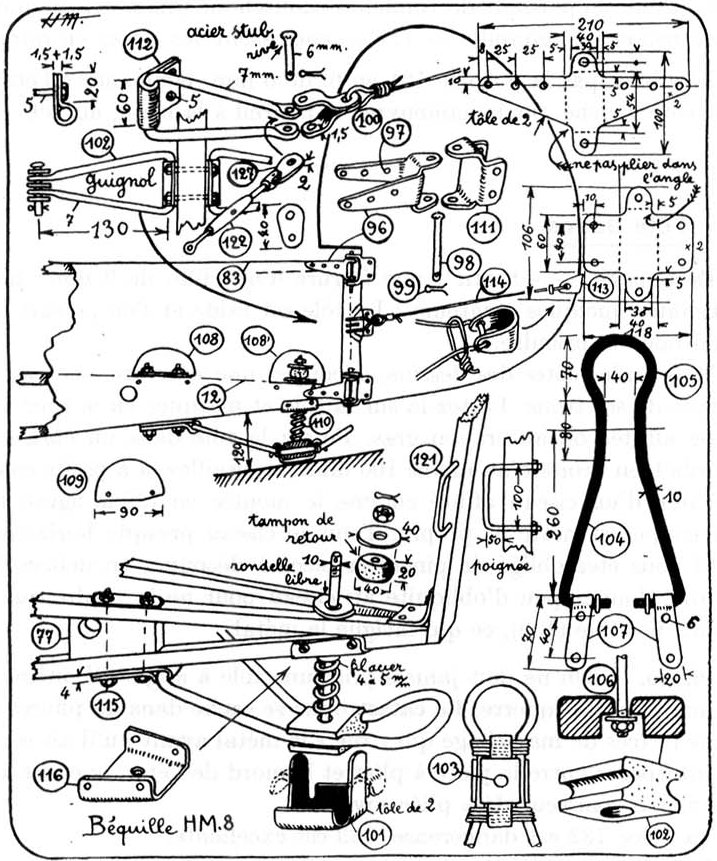
\includegraphics[width=\linewidth]{fig-35.jpg}
  \caption{Rear landing gear}
  \label{fig:thirtyfive}
\end{figure}

Fitting \circled{112} carries the horns \circled{102}, made of 7mm
drawn rod, flattened at the ends and pierced to receive a little steel
axle, which holds fittings \circled{100} and \circled{127} together.
These horns are wired to the trailing edge \circled{113} of the rudder
--- at the location of a rib gusset --- with a 2.4mm cable
\circled{114}.

The pair of cables that connect the horns to the control stick are
adjusted by turnbuckles \circled{122}.

The tailskid is formed like a triangle of 10mm drawn soft steel wire
\circled{104} with the ends bent in and aligned on the same axis to go
into the 2mm sheet steel fittings \circled{107}.

The fittings \circled{107} will be fastened with bolts \circled{115}
of 6mm threaded rod, taking care to align the heavy wire loop
\circled{106} with the center line of the fuselage.

An opening \circled{108} cut in the sides provides access to the nuts
fastening the bolts \circled{115}, which clamp a plate of 2mm sheet on
the piece of hardwood 77.  Small covers \circled{109} made of 0.6mm
aluminum sheet screw over the opening.

The shoe \circled{101} of 2mm sheet steel is attached to the loop
\circled{105} by a hardwood wedge \circled{102}, pierced with a hole
\circled{103}, which receives a 10mm rod \circled{106} with a nut,
holding a spring \circled{110} which yields at 40kg (12 turns of 35mm
steel wire, like 6mm motorcycle seat springs); then a sheet-metal
bracket \circled{116},secured under the fuselage by 4 good wood
screws; a washer 2cm thick; a rubber donut 40mm in diameter; a nut;
and a pin \circled{117}.  All this forms the shock-absorber.

Do not forget the handle \circled{121} of 6mm wire, bolted to the left
side, which eases ground-handling.

\sectline

\subsection{Interlude: Mild steel sheet}

\textbf{Cutting} --- Cutting a fitting from a sheet of 2mm steel can
intimidate some amateurs.  The sheet is stiff, and one doesn't know
where to start.

Cut out a cardboard fitting made to the dimensions in the drawing, and
pierce it with holes.  Fasten it to the steel sheet and mark the
outline with sharp chalk or a grease crayon.  Clamp the sheet in a
vise with straight edges of at least 100mm, and cut it with a
sharpened chisel as shown at \circled{129} in figure
\ref{fig:thirtysix}.  This will make a clean, accurate cut.  Hold the
chisel almost horizontal.

\begin{figure}
  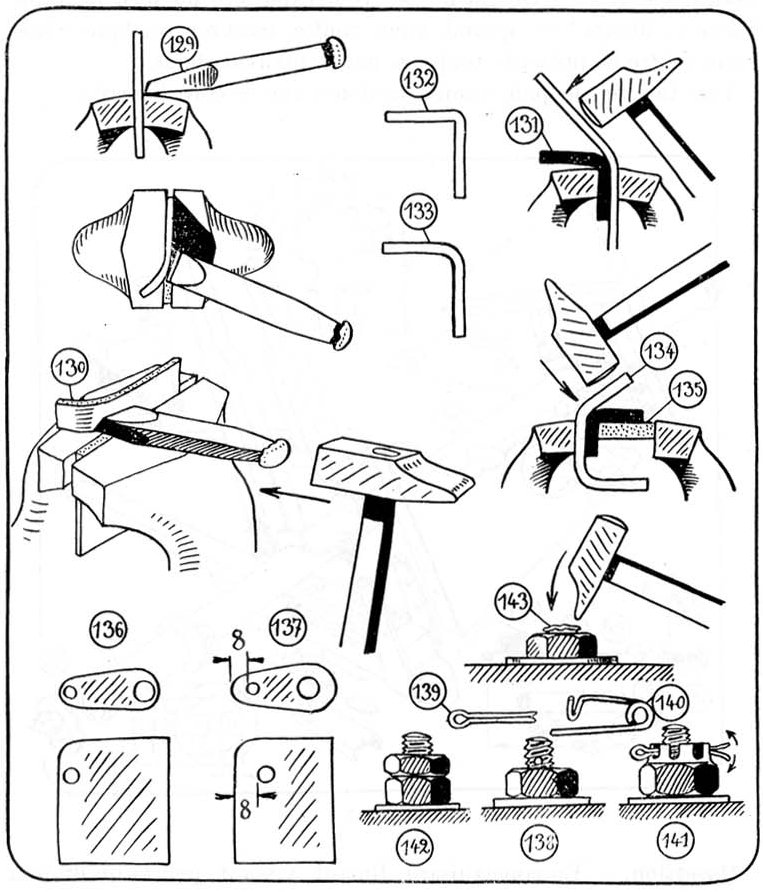
\includegraphics[width=\linewidth]{fig-36.jpg}
  \caption{Fashioning sheet steel fittings}
  \label{fig:thirtysix}
\end{figure}

\textbf{Bending} --- One should never bend steel sheet at a sharp
angle, even the smallest piece.  Disaster hides in these bends,
because the excessive hammering ``kills'' the metal before it has been
used.  To avoid it, place between the piece to be bent and the jaw of
the vise a piece of the same thickness that has already been bent
correctly.  \circled{132} is a dangerous piece, but \circled{133} is
excellent.

To bend in a ``U'' \circled{134}, put in a piece as a spacer
\circled{135}, \textit{e.g.} an old, worn-out file.

\textbf{Drilling} --- Drill away from the edges.  When my drawings do
not specify the dimensions --- I didn't draw them for fools! --- leave
at least 8mm between the hole and the edge of the fitting, and if
possible 10mm.  Leave an equal amount all around the hole.
\circled{136} is very bad, but \circled{137} is good.

\textbf{Fastening} --- On an airplane, all bolts must be secured.
When the part is frequently disassembled, the nut \circled{138} is
secured with a pin \circled{139} or \circled{140}.  In more precise
assemblies, use castle nuts \circled{141} or lock nuts \circled{142}

When the bolt is not intended for disassembly, a few hammer strokes
will roughen the threads \circled{143} of the bolt that protrude about
2mm beyond the nut.  Before disassembly, a light filing removes the
roughness and allows the nut to be removed.

Not a nut, not an axle, not a turnbuckle may be forgotten.  If you
neglect to tighten a dozen nuts on purpose, none will come off.  But
if you forget one, and it is important, that is the one that will
desert you: you will drop parts all over the landscape!  Nature abhors
a vacuum and despises order, and will have its revenge\ldots For the
same reason, if you drop a nut, it immediately becomes invisible ---
where is it? --- Cuddled up behind a table leg.  Never anywhere
visible!  When you want to measure anything, your ruler is always at
the far end.  Bread always falls butter-side down!

\textbf{Obsession} --- In building, filing, and fastening, remember
that one day soon the piece you are working on will be what holds you
suspended in the void, a thousand meters above the ground\ldots

\subsection{Front landing gear}

The axle is a $36\times40$ tube \circled{144}
\textit{(fig. \ref{fig:thirtyseven})} 1200mm long, filled with another
reinforcing tube, $31\times35$ 800mm long.  This is 4mm thick in
total, and weighs 4kg 300g.  It is heavy --- very heavy.  But it's
solid!  The axle won't bend.  You won't have to worry about beating
your landing gear into a curve rolling over the clods.  Do not repeat
the author's mistakes --- \textit{only one tube is not enough}.

\begin{figure}
  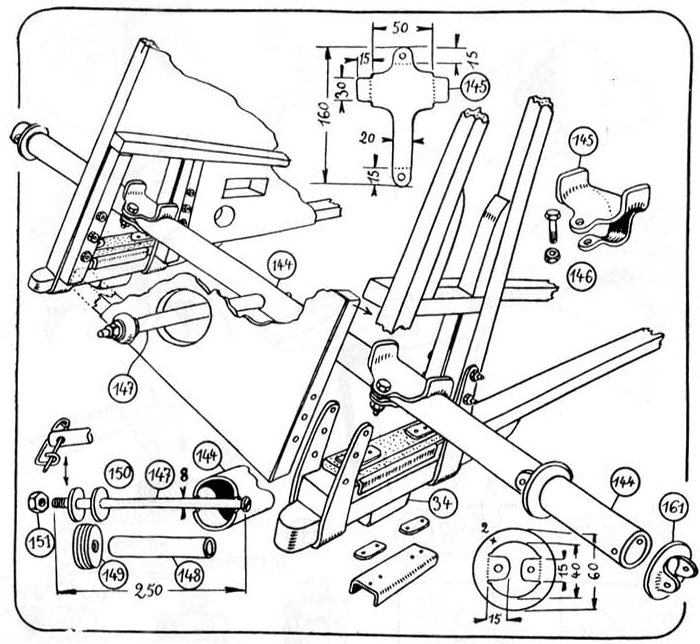
\includegraphics[width=\linewidth]{fig-37.jpg}
  \caption{The axle and its placement}
  \label{fig:thirtyseven}
\end{figure}

1mm play between the tubes allows you to assemble them; if you made
them fit tightly, you could not fit them together.  I do not recommend
a wooden sheath, which, while lighter, prevents neither bending nor
breakage.  Its elasticity allows the metal to fatigue, and your axle
will eventually break from a light bump.

A collar \circled{145} of 2mm sheet is tightened onto the tube by its
6mm bolt \circled{146}.  This collar prevents the tube from slipping
through the bungee cord, just as the block \circled{34} holds it under
the wooden pad under the cabin.

Neither drill any holes nor do any welding on the axle just now.

An 8mm rod \circled{147} crosses the axle in the middle.  On it are,
in order, a tube \circled{148} of rolled 1mm sheet, a plate washer
\circled{150}, rubber washers \circled{149}, another washer
\circled{150}, and finally a nut \circled{151}.  This prevents the
axle turning by bearing on the front floor through hole \circled{50}

\begin{figure}
  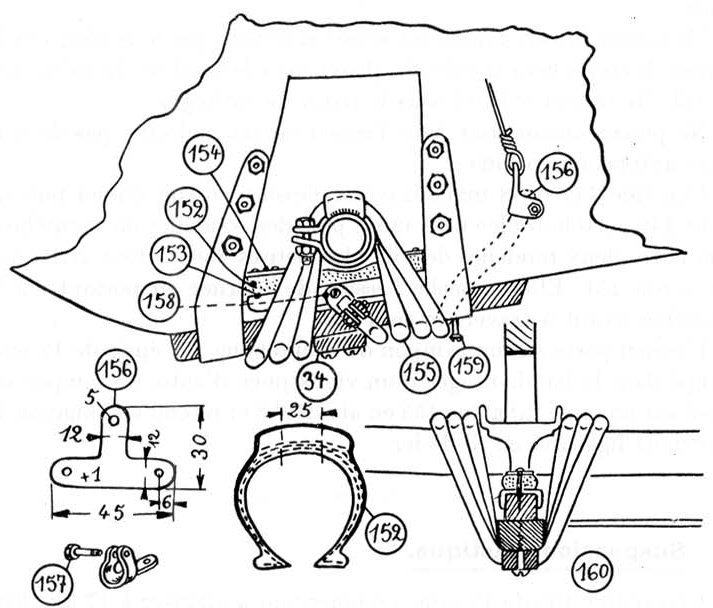
\includegraphics[width=\linewidth]{fig-38.jpg}
  \caption{Rubber pads and bungee cord}
  \label{fig:thirtyeight}
\end{figure}

The axle rests on a 12mm-thick rubber pad \circled{152} cut from the
tread of a used car tire.  This pad is placed on a folded sheet of
0.6mm aluminum \circled{153} and held to the longeron \circled{12} by
two steel wire ligatures \textit{(fig. \ref{fig:thirtyeight})}.

\subsection{Bungee suspension}

A 12mm bungee cord \circled{155} 1m 90cm long, which starts to stretch
at 17kg, is clamped at each end in a fitting \circled{156} of 1mm
sheet metal held by a 4mm bolt \circled{157}.  \textit{Fastening}: One
end of the bungee cord is fixed under the axle by a $4\times20$ screw
\circled{158}.  The bungee goes behind the block \circled{34}, and
then six times around the axle and under the pad as shown in the
figure.  It is stretched so that it extends a little.  Leave no slack.
The other end fitting is attached to a 2mm wire, which is fastened
somewhere under the seat bottom.  A screw, \circled{159}, prevents the
rearmost strand from sliding.  Be certain that the axle, in the play
allowed to it, does not rub on an immobile strand of bungee.

Before cutting the bungee cord to length, tie it with string two
times; then cut it with a sharp knife between the ties.

From the front, the suspension appears as at \circled{160}, where we
see the axle, its collar, the rubber pad, the folded sheet, the
longeron, its reinforcement pad, and its lower block with three
strands of bungee on either side, which makes 12 total strands of
suspension on either side of the cabin.  The machine can roll on a
single wheel without stretching the bungee cord shock absorber.

The wheels are held at the end of the axle by the washer/collars
\circled{161}, held by a horizontal 5mm bolt, cut from 2mm sheet
according to \circled{162}\footnote{I am unable to find this reference
  number on any drawing, but \circled{161} is in
  Fig. \ref{fig:thirtyseven}, and includes layout details for the
  washer collar in question.}.  15mm long $40\times44$ tube ends would
also serve.  Insert a washer between the wheel and the sleeve.

This landing gear is not as smooth on rough ground as a triangular
frame with coil springs, but it is simple, rustic, easy, light --- and
aerodynamically sound.

Work: 1 day; weight with wheels: 12kg.

\subsection{Wheels}

I strongly recommend $450\times10$ tires, not too inflated, which
absorb most of the normal shocks due to rough ground.  The big shocks
are handled by the bungee cord.  Inflate the tires so they barely hold
their round shape.

Grease the axle often.  Amateurs have often had them seize due to
negligence.

These wheels are small; the belly of the fuselage is only 14cm from
the ground.  It seems week.  Practically, I have never had trouble.
This should not, however, prevent you from carefully surveying the
starting ground and beating the most prominent molehills down with a
shovel.

I suggest that manufacturers give thought to aircraft of about 200kg
gross weight, and make tires weighing 1kg with hubs the same weight.
It must be possible.  They'd sell like hotcakes!

We would also need a spherical tailwheel 140mm in diameter.

\subsection{Control stick}

A tube \circled{163} \textit{(fig. \ref{fig:thirtynine})} passes
straight through the fuselage below the rectangular hole 26
(Fig. 51\footnote{This figure does not contain any such hole.}).  You
will have to use a brace and bit to drill a hole \circled{164} as seen
at \circled{165}, and use a rasp to fit it to the diameter of the
tube, \textit{i.e.} 24mm.

The middle of the tube \circled{163} is held between two wedges
\circled{166}, surrounded by two cheeks \circled{167} of 2mm steel,
all held by four 5mm bolts.  The control stick \circled{170} pivots
between these two cheeks on a 6mm bolt \circled{168} and two 1mm
washers \circled{169}, reinforced at this point with a sleeve.
Riveted at the top of the stick is a hook \circled{171} of 2mm sheet
metal, which allows a secure grip.

\begin{figure}
  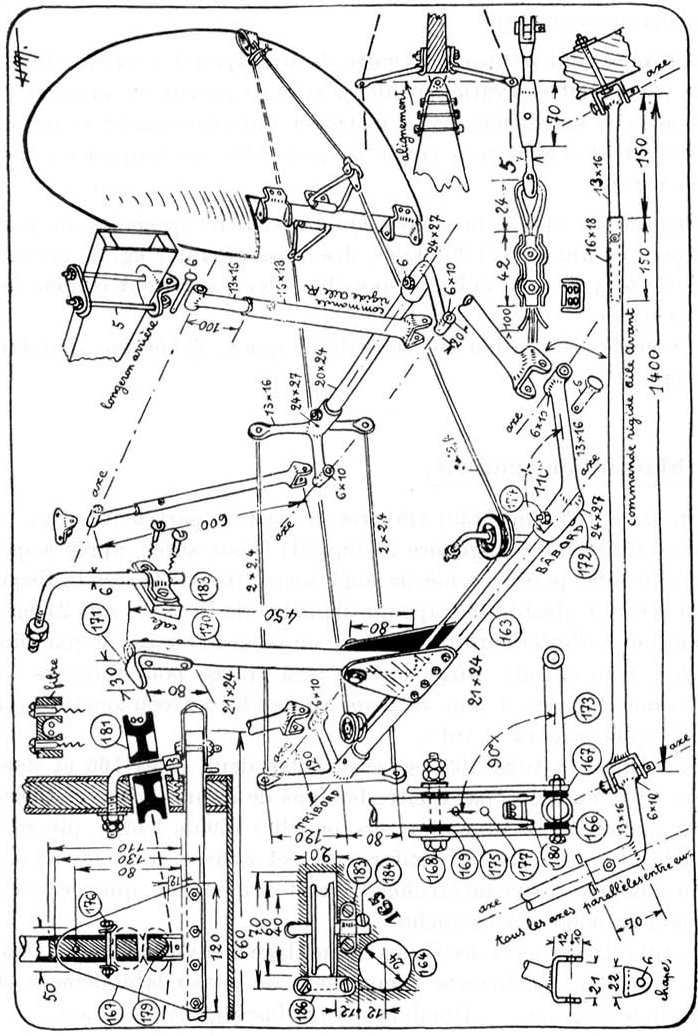
\includegraphics[width=\linewidth]{fig-39.jpg}
  \caption{Layout of control system}
  \label{fig:thirtynine}
\end{figure}

The tube \circled{163} extends beyond the fuselage sides by about
50mm.  Two collars \circled{172} prevent it from slipping laterally,
\textit{without play} if at all possible.  There must be washers
between the fuselage and the sleeves.

These sleeves also bear the horns \circled{173}, and are fastened to
tube \circled{163} by a 6mm bolt \circled{174}, so that the horn forms
an angle of about 90$^\circ$ with the handle.

The horns, one on each side, for control of the wings, will be bound
to them by a rigid pushrod.

The rudder control can be hooked up now.  Two 2.4mm steel cables, 5m
long, will be passed through the 6mm hole \circled{175} in the handle,
and fixed in the middle by a 4mm bolt \circled{176}.  Each double
strand will cross the other in the 5mm hole \circled{177}, and then
again in notch \circled{178}.  The handle will have been filled with
hardwood rubbed with paraffin, flush with the base of the handle.  The
wood and metal notch will be filed in a circle according to 179.  A
4mm rivet \circled{180}, flush with the handle, prevents the cables
from escaping the notch.  A drop of oil will prevent cable wear, but
you must keep an eye on it and replace the cables according to need.

Each double strand 2m 50cm long, runs over the pulley \circled{181},
which is of cast iron with a very wide groove, no less than 40mm, and
can be bought at any hardware sellers' --- rotating on the 6mm shaft
\circled{182}.  A fuselage nut inside the fuselage on one end, a
bracket \circled{183} on the other, and a $5\times25$ screw
\circled{184} below the bracket secure this shaft at a slight tilt
(with a wedge under the end of the shaft) to align the cable's path
with the base of the handle.

Finally, the double strand will join the turnbuckle \circled{122}
\textit{(fig. \ref{fig:thirtyfivw})} where it is attached by a cable
clamp \circled{123} designed for 4.5mm cable.  Tie each loose end and
join them both to the cable.  Leave 50---100mm excess.

A small 2mm sheet \circled{185} flush with the pulley and applied by
two screws will prevent the cable from escaping and getting caught if
it were to become loose.  Wise precaution --- you never know!  The
tendency of a cable to stick is powerful, and if there are only two
pulleys in the Pou-du-Ciel, it's two pulleys too many!  A million
bucks to the one who can get rid of these two pulleys!

The front-wing control horn \circled{420} is connected to the
rear-wing horn \circled{421} by two 2.4mm cables \circled{422}, each
doubled, like those of the rudder\footnote{The reference numbers
  \circled{420}---\circled{427} in this paragraph and the following
  ones are not to be found in the figures.  Their referents are mostly
  obvious, however.}.

This rear horn has a projection \circled{423} which moves a pushrod
\circled{424} carrying a projection \circled{425}.  The shaft turns in
a waxed hole drilled in the filler piece, \circled{77}.

The two projections \circled{423}---\circled{425} control the rear
wing by two arms \circled{426} pivoted on clevises \circled{427}
bolted to the small spar of the rear wing.

Time: 2 days.  Weight: 2.3kg.

\subsection{Cabane struts}

The cabane is the steel-tube pylon which supports the wing and holds
it in position with regard to the fuselage before it is secured by the
bracing wires.

It is made \textit{(fig. \ref{fig:forty})} of two $17\times20$ tubes
\circled{187} welded onto two 2mm cheeks \circled{188}, which are
separated by a block of hardwood \circled{189} and fastened by two 6mm
bolts.  If welding is not available, bolt as at \circled{190}.  This
is the top of the cabane.

The bottom of the cabane, slightly curved while heated red-hot and
filled with hardwood, are held in U-shaped brackets \circled{191} of
2mm steel by a 6mm bolt.  These are linked to another bent fitting
\circled{192} by two 6mm bolts, enclosing the cross-member
\circled{67} and giving the structure great strength, fitting
\circled{192} being bolted on its other side to the three members
\circled{14}, \circled{15}, and \circled{16} of the undercarriage.

It would be better for the lower ends of the cabane struts end with a
welded transverse tube \circled{193}.

The top of the cabane is fixed in place by a tube \circled{194} about
300mm long --- to be determined at the time of adjustment of the wing
--- and which is fastened, top and bottom, on 30mm tubes \circled{195}
of rolled 1.5mm sheet. The tube-axis of the foot is clamped between
two brackets which will be bolted to the engine when it is installed.

\begin{figure}
  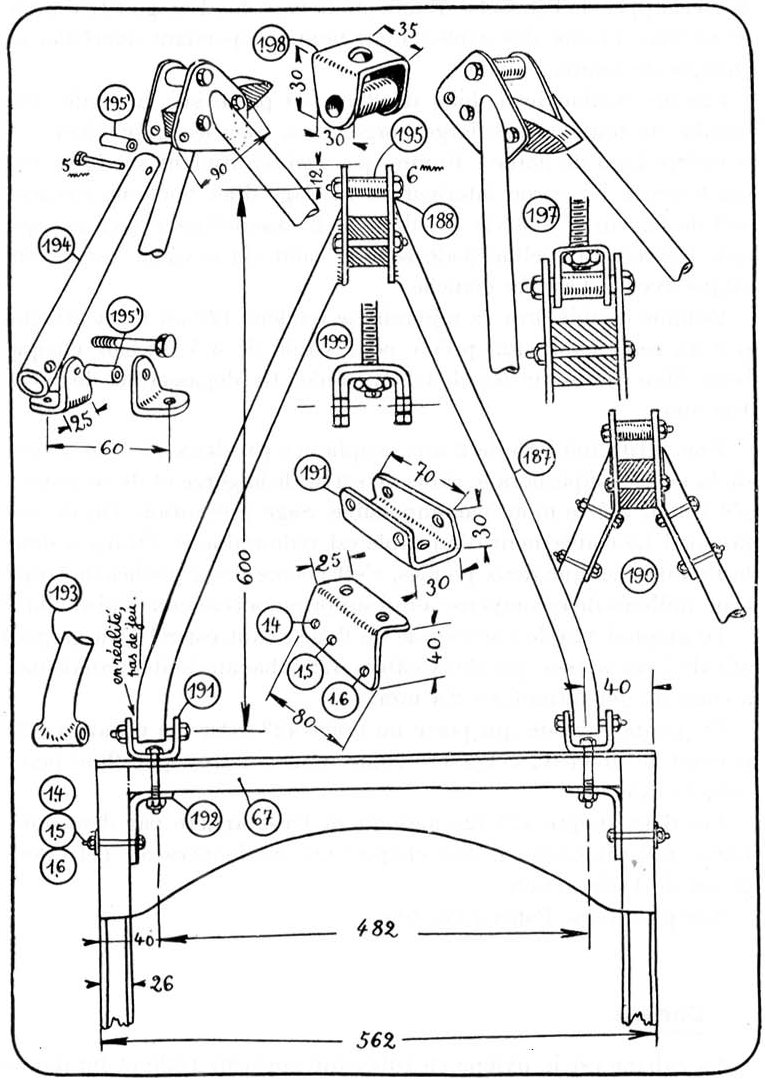
\includegraphics[width=\linewidth]{fig-40.jpg}
  \caption{Layout of cabane struts}
  \label{fig:forty}
\end{figure}

The small tube \circled{195} at the cabane top forms the axis around
which the wing rotates.  To achieve this, a 200mm bolt \circled{197}
of threaded 10mm rod runs through the wing vertically and retains the
U-fitting \circled{198}, which is welded to a tube of rolled 2mm
sheet.  Pivoting is provided by these two tubes rotating one over the
other --- one attached to the cabane, the other secured to the wing.
If welding is unavailable, a fitting without the tube but of doubled
sheet as shown at \circled{199} will suffice.  Tube \circled{195} must
be fastened, and adjusted so the fitting \circled{197} moves freely
without lateral play.  Precise fitting of the tubes is unnecessary; 1
or 2mm play will not matter as long as they are approximately round.
A drop of oil will fix everything.  Let the engineers laugh\ldots Why
bother if it's not necessary?

Time: 1 day.  Weight: 1.5kg.

\chapter{Wings! Wings!!}

\section{Wingspan}

My intent was to give the amateur a Pou-du-Ciel project that he can
build in his apartment.  A space 4$\times$3m should have sufficed.
The fuselage, the rudder, the rear wing\ldots all possible.  But what
about with this bothersome front wing?

Four meters wingspan would have been fine.

I tried.

A first, flat-bottomed airfoil carried me to the flats of the Aisne
valley poplars.  The engine, running full out, quit.  I came down in a
60m meadow surrounded by walls, with an apple tree and a horse.  I hit
a manure pile without much damage.  Another more curved profile got me
up to 100 meters.  It climbed like an old man climbing stairs: very
slowly, with much huffing and puffing.  It made me want to pedal!

So much for 4 meters.  I stretched the wing to 6 meters and the
highlands, the towns and the forests dropped away beneath my wheels,
the landforms flattening before me.  It was too good to abandon.  For
a span of 6 meters, the amateur will have to make what shift he can.

After a few mishaps, I settled on an autostable airfoil.  By ongoing
study of the two wings' interactions, I was able to modify the section
given in my former book to improve the performance of the Pou-du-Ciel
1936.

\section{Forward wing}

The structure of the wing \textit{(fig. \ref{fig:fortyone})} consists
of 18 ribs strung on a 6m main spar \circled{200}.  A smaller 5m spar
\circled{201} is threaded with the tail ends of 12 ribs, all the same;
the three ribs numbers 7, 8, and 9 on each side are different because
of the planform of the wing.

\begin{figure}
  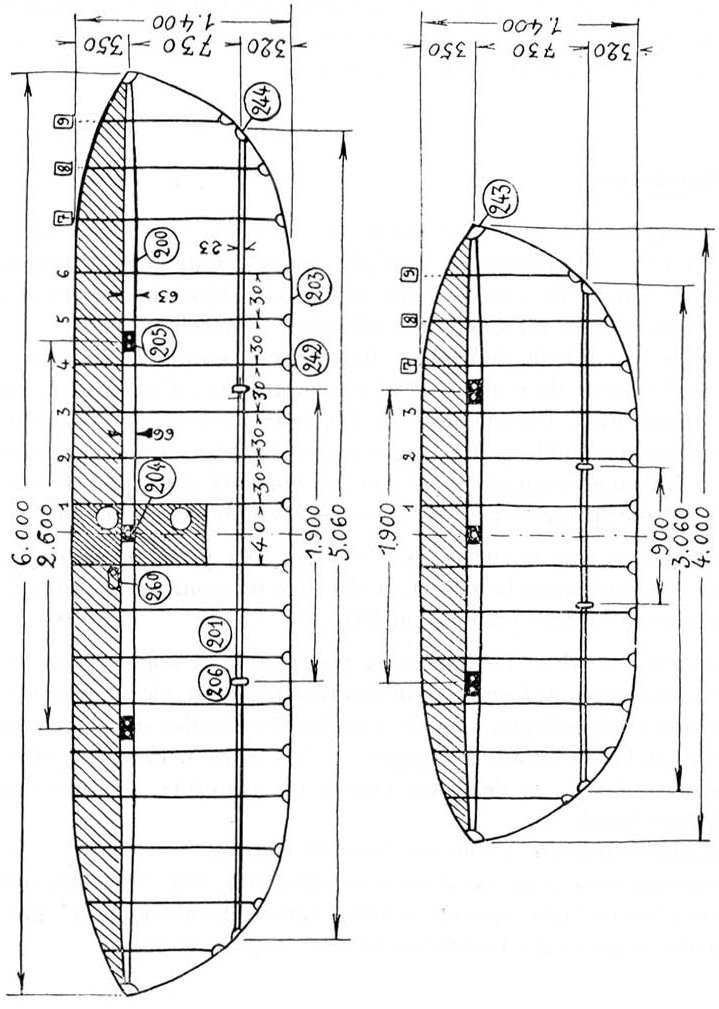
\includegraphics[width=\linewidth]{fig-41.jpg}
  \caption{Overview of wing structure}
  \label{fig:fortyone}
\end{figure}

The trailing edge \circled{203}, made of three glued strips, and the
small spar triangulate the frame that needs no additional stiffening.
Thus, inside the wing, except for the nails for the plywood, there are
no metal parts: no fittings, no wires, no turnbuckles.

The center of the wing is supported on the cabane by a block
\circled{204}, while a system of struts fitted to the wing at
\circled{205} fix it firmly along a pivot axis
\circled{204}---\circled{205}.

The pivoting motion is regulated by the rod which connects the control
horn \circled{173} of the control stick to the rear spar, on which
this rod is fixed to two shims at \circled{206}.

\sectline

\section{Main spars}

The spar \textit{(fig. \ref{fig:fortytwo})} consists of two
15$\times$60 caps \circled{207}, \circled{208}, curved to meet at the
tips and held in shape by two vertical-grain plywood webs
\circled{210}.  The spar is 150mm deep.

\begin{figure}
  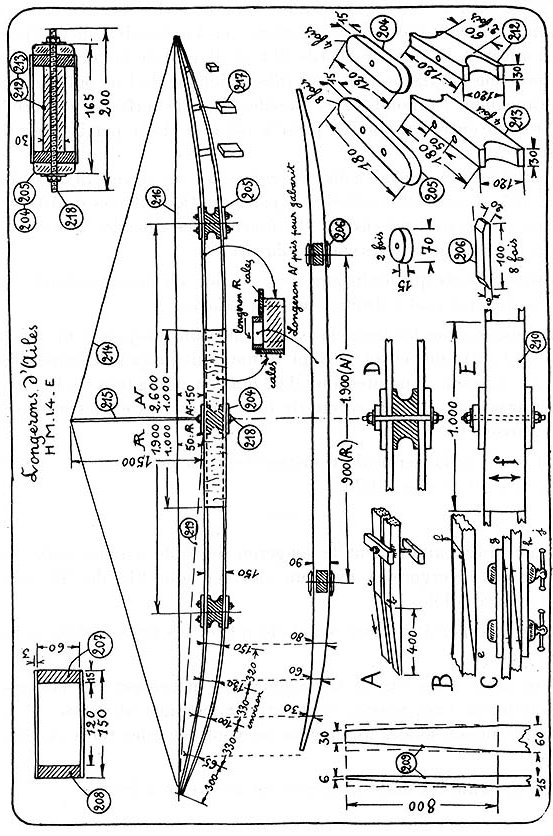
\includegraphics[width=\linewidth]{fig-42.jpg}
  \caption{The spars}
  \label{fig:fortytwo}
\end{figure}

It can be hard to find 6mm lengths of fir free from knots; their
length also makes them inconvenient to ship.  So let's begin with two
lengths of 3m 20cm which can be joined with a scarf joint.  Plane the
ends of the two 15$\times$60 boards together, as at \textbf{A}, to a
slope 400mm long, clamping them firmly to the workbench.

Make sure the surface \textit{a b c d} is flat and even.  After you
plane, use a file or fine rasp to remove the gloss.  Form the other
ends as at \circled{209}.

Join --- \textbf{B} --- the bevels with plenty of glue and align the
two lengths of wood well, immobilizing them with two nails in
\textit{e} and \textit{f}.  Tighten --- \textbf{C} --- the joint,
protected with double sheets of newsprint, between two blocks
\textit{g} and \textit{h}, in the jaws of a vise, strong carpenter's
clamps, or pressed with very heavy weights.

Let dry 12 hours in summer, 24 in winter.

Then prepare for each wing the wedges \circled{204}, \circled{205},
\circled{212}, and \circled{213}, which can be in excellent fir or in
beech.  All holes are 11mm.  Also prepare 5 10mm threaded rods 200mm
in length.

\sectline

\subsection{Assembly}

Having removed the two spar caps from their clamps, and cleaned up all
four sides, drill an 11mm hole in the middle, and two holes, 50mm
apart at 1.3m to either side of the middle.  More precisely, these
double holes will, on the upper cap, be 3mm closer to the middle.

Put the two spar caps on two sawhorses and join them with plenty of
glue --- as seen at \textbf{D} --- by the block \circled{212}, under
the also firmly-glued plates \circled{204}, and by the 10mm threaded
rod 218 and its two nuts with washers.  10mm lock nuts are sufficient
--- and lighter than normal nuts.  Make sure the spar caps are
parallel to each other from end to end for now.

Then glue --- as seen at \textbf{E} --- on each side, two strips
\circled{210} of 3mm plywood, 150mm wide over \textit{f}, and 1m long
(for both wings).  Using a rope or a 2mm wire \circled{214} and a 1.5m
rod \circled{215} of wood, bamboo, tube, or the like, flex the tips of
the spar caps upward so a string \circled{216} stretched between the
wingtips passes 150mm above top of the newly-boxed center section.

Insert the blocks \circled{213} with plenty of glue.  Tighten them
under the plates \circled{205} using their 10mm threaded rods, but
\textit{do not glue the plates}.

Little temporary blocks \circled{217} will hold the spar caps spread
toward the tips, according to the approximate dimensions shown.

Make sure the bending of the spar caps, verified by string
\circled{219}, is approximately the same on both sides.

Cover both sides of the spar, using 3mm plywood up to 1.3m either
direction from the center, then 1.5mm for the remainder, and nail with
fine 8mm nails every 15mm in a zigzag pattern.  Use butt joints, or,
if you use scarf joints, do not allow extra thickness.

In all, this 6-meter spar used a little over 1 square meter of
plywood, and weighs 7 kilograms.

\sectline

Build the spar of the rear wing the same way, but to a span of 4
meters and with a distance under the string \circled{216} of 100mm.
This spar weighs 5 kilograms.

Let dry 12 hours before removing the threaded rods and the plates
\circled{205}.

You will be amazed at the stiffness of these spars.  They give the
impression --- and an accurate impression it is --- of truly solid
work worthy of all your confidence.

These two spars can be built in less than two days.

\sectline

\section{Rear spars}

The small rear spars of each wing consist of two 10$\times$20 spar
caps joined by a single web of 1.5mm plywood.  They are 90mm tall.
They are built by taking the large spars for a template and giving
their lower cap the same shape as the lower cap of the large spar.  To
aid in that, 6x12 strips should be nailed \textit{under} the caps of
the latter and beyond it by 6---8mm on the edge.  With its blocks
properly arranged, the small spar will take on the dimensions given in
the figure.  Do not forget the side reinforcement plates
\circled{206}.

\sectline

\section{Ribs}

The propeller\ldots is the summation of Aviation!

The rib\ldots is the summation of the glider!

You can mess up a lot of things in an airplane: fuselages that are
misshapen, heavy, or spindly; crinkled cowlings; twisty tubes\ldots
the curvature of the wing, however, must remain unspoiled.  Several
countries have established laboratories to scientifically study
airfoils.  They have spent hundreds of millions!  The best airfoils
that have been discovered look like birds' wings, and the thin section
has not yet spoken its last.  Henri Mignet also has his aerodynamic
laboratory (which cost him 600 francs!), and gave birth to an airfoil
his own way, resembling an autostable pre-war section --- O Progress!
Its sharp leading edge earned him some sarcasm, but that was not its
failing.  Its flaw was its hollow underbelly, which, in the attempt to
provide autostability, killed its lift.

So I sneaked into a hanger with many French, English, and German
airplanes, with my ruler in my hand and a pencil behind my ear.

I, tired of jostling my own airfoil back and forth, was in the
presence of a simple profile: rounded leading edges, flat bellies,
back gently curved, trailing edges raised slightly\ldots I
superimposed several profiles and took an average, aiming at lift
rather than speed\ldots

My friend Robineau broke his old wing and built a new one with the new
airfoil; we have experimented with it for a long while.  Here, then,
is the new Pou-du-Ciel.

My old airfoil with its pointy beak and wavy tail are now forgotten in
the cabinet.

The sacrosanct airfoil is now supported by a plywood sheathing on the
rounded leading edge.  The amateur will have 6 hours more work, but
the difficulty is not great.  The little clever ones behind the
barriers will not laugh anymore: here we are working by the book, and
the bad guys will look a little green at how disgustingly good the
performance has become.

We have too much power now!  We may soon content ourselves with a
motor bike engine\ldots and the dearest of my dreams will soon be
realized\ldots

\begin{center}
  {\large \textbf{Aviation for the Little Guy!}
    
    \textbf{Ha! Ha!!}}
\end{center}

\subsection{Ribs}

Cover a board 300$\times$1500 with white paper and draw the profile of
the rib as follows:

Draw a straight line \circled{220}
\textit{(fig. \ref{fig:fortythree})} 50mm above the bottom edge.

\begin{figure}
  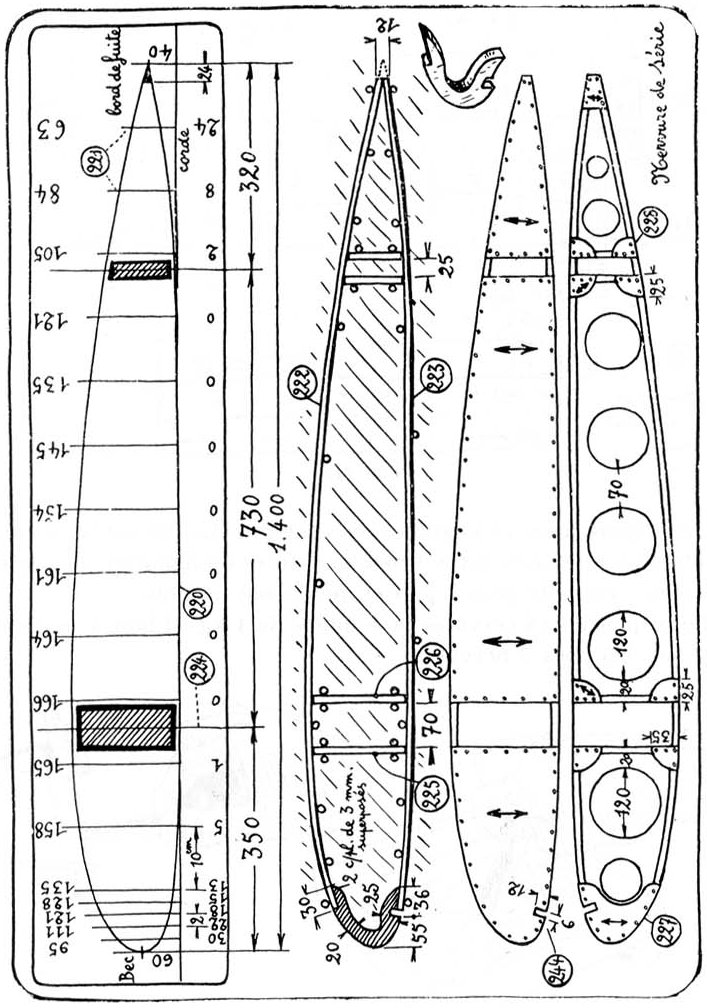
\includegraphics[width=\linewidth]{fig-43.jpg}
  \caption{The standard rib pattern}
  \label{fig:fortythree}
\end{figure}

Draw upon it 15 perpendicular lines \circled{221} spaced 100mm apart
and mark them according to the dimensions inscribed: 60 marks the
front of the leading edge, while 13 and 135 mark the respective
distances from the line \circled{220} of the belly and back of the
airfoil.  Continue that way to the tail of the rib, whose trailing
edge is 40mm above the line.  This line \circled{220} forms the
\textit{chord} of the wing.

Join the points you have made, and you will have a section view of the
shape of the thicknesses of the wing: the airfoil.

Two cap strips \circled{222}, \circled{223} in 6$\times$12 are held
along the broken line with 2mm nails whose heads you have cut off.
The rounded leading edge and is cut from a 12mm-thick board.

350mm back from the leading edge, mark a line
\circled{224}\footnote{Which is not numbered on the diagram but can be
  identified by its description.}: it is the axis of the forward spar
bolts.  Place a 6$\times$12 member on either side of this line,
leaving a 70mm space.  This is where the spar slips through the ribs.

Connect the two cap strips \circled{222}, \circled{223} with a 1.5mm
plywood web, observing the marked direction of the grain.  Hold with
8mm brads every 25mm.

Remove the rib from its jig; it has its shape.  Nail on the other side
the gussets \circled{227} and \circled{228}.

Build 19 ribs.  The nineteenth, sanded and varnished, hang somewhere
prominent in your office, to remind you of these hours of joyful labor
later on.

With a hole cutter, lighten the web --- it's no trouble.  You remove
50 grams per rib, which is nothing.  But repeated, it eliminates a
kilogram --- which is very ``Aviation''!

Each rib weighs 230 grams.  It takes 10 minutes to nail one up.

The non-standard ribs \circled{7}, \circled{8}, and \circled{9}, of
which you make four each, will be drawn and built in the same way;
following Figure \ref{fig:fortyfour}.

\begin{figure}
  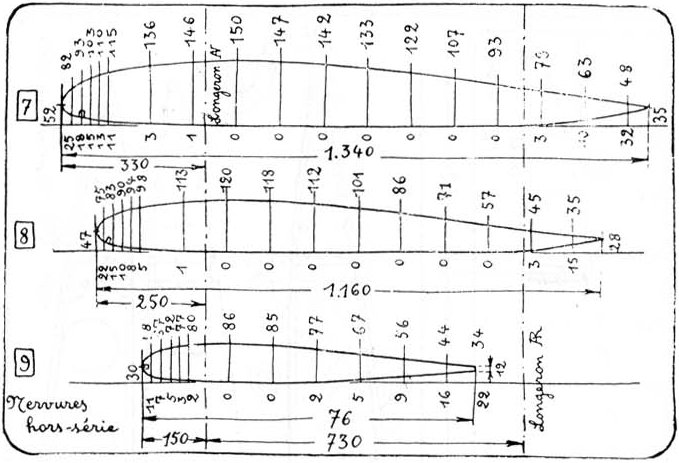
\includegraphics[width=\linewidth]{fig-44.jpg}
  \caption{Non-standard rib pattern}
  \label{fig:fortyfour}
\end{figure}

Webs and cap strips are prepared in 5 hours.  The 31 ribs are nailed
up in a single afternoon.  A few hours of sanding\ldots a day and a
half, that's all.

The 18 ribs weigh less than 4kg together.  1m\textsuperscript{2} of
1.5mm plywood makes seven ribs.

\subsection{Nailing}

\begin{figure}
  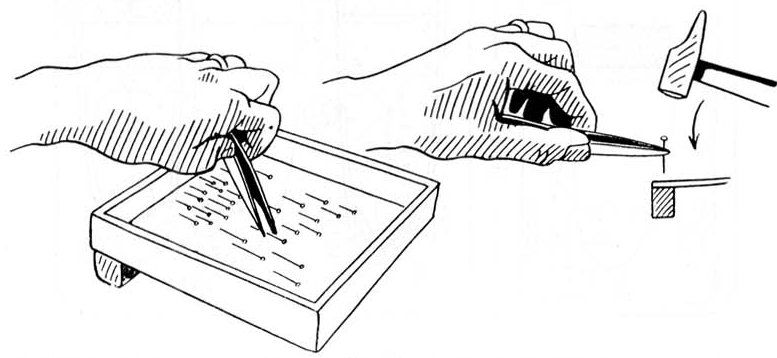
\includegraphics[width=\linewidth]{fig-45.jpg}
  \caption{Using a tilted nailbox and tweezers}
  \label{fig:fortyfive}
\end{figure}

You will be able to calmly drive two nails in three seconds using a
tilted nailbox, which, shaken by nearby hammering, will orient all the
nails with their heads to your right.  With a pair of tweezers you
will easily grab them and place them one by one under the hammer.
With the first blow, the nail is set.  Remove the tweezers.  Another
blow, and the nail is flush.

You'll be more efficient, and you won't hit your thumb and forefinger
\textit{(fig. \ref{fig:fortyfive})}.

Keep the glue pot well away from the nailbox: Sometimes, in the heat
of battle, you dip the glue spreader into it and remove a beautiful
glob\ldots unless, distracted, you stick your fingers into the cold,
sticky mass\ldots

The Pou-du-Ciel sprouts its two wings in one week.

\section{Wing assembly}

Set the spars across two sawhorses, perfectly parallel and level, with
the tips pointing down.  Thread the standard ribs \textit{1, 2, 3, 4,
  5, 6} in order, their bellies up, on each side of the glued central
block \circled{204}.  Each rib is glued and nailed directly to the
spars by two 20mm nails \circled{230}.

\begin{figure}
  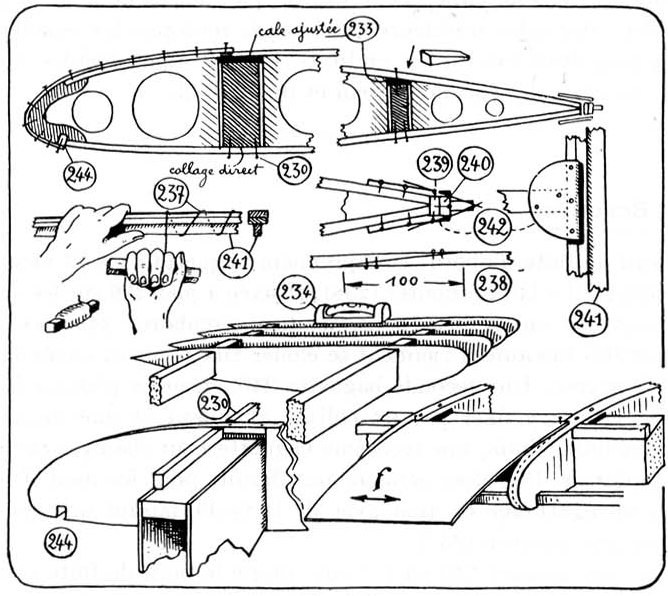
\includegraphics[width=\linewidth]{fig-46.jpg}
  \caption{Assembling the wings}
  \label{fig:fortysix}
\end{figure}

The two innermost ribs are spaced 400mm apart; the others 300mm
\textit{(fig. \ref{fig:fortyone})}.

Turn the whole thing upside-down and fit the blocks \circled{233} with
plenty of glue between the ribs and the spar caps.  Then nail them so
all the rib bellies are parallel, checking with a spirit level
\circled{234}.

Glue and tighten by their threaded rods the plates \circled{205},
\circled{206} \textit{(fig. \ref{fig:fortytwo})}.  These plates are
level with the ribs above and below the wing.  Glued parallel to the
inner blocks \circled{213}, these reinforce the spar caps, which are
pierced through here by the threaded rods.  The wood of these plates
must be excellent quality with perfectly straight grain.

\sectline

\section{Leading and trailing edge}

Trailing edge first.  Take a first strip of wood 6$\times$12, scarfed
if necessary \circled{238}, and fix it flat \circled{239} on the tails
of the ribs between two half-circle gussets \circled{242}.  The two
beveled ends are nailed to the ends and back of the main spar.  A
second strip \circled{240} is placed flat on the first and held with
plenty of glue and a dozen fine nails.  Finally, a third strip, placed
on its edge, reinforces them.  Nails alone are not sufficient to hold
these; they must be tied with string, making a turn every 30mm or so
\circled{237}.

A large 1.5mm plywood gusset unites the trailing edge with the ends of
the main spar.

If you fear that the strips may break in bending, especially the
third, moisten them with a damp cloth for 5 minutes before you fit
them.

\subsection{Leading edge}

A 6$\times$12 strip is laid from end to end in the notches
\circled{244} cut under the nose of each rib.  Pieces of 6$\times$12
strip are then placed on edge \circled{230}\footote{This refers to
  \circled{230} at the bottom of Figure \ref{fig:fortysix}, not the
  one at the top.} between each pair of ribs along the front of the
spar.  Then wrap the rounded top of the ribs with 1.5mm plywood, the
grain of which should run along the wingspan, gluing from
\circled{230} to \circled{244}.  It is wise to only cover one bay
(\textit{i.e.} 300mm) at a time, either butting the plywood sheets at
the middle of each rib, which gives 6mm gluing area for each, or by
overlapping slightly beveled edges; \textit{i.e.} a scarf joint.  This
covering must be very firmly bonded, so we advise against covering
three or four bays with a single sheet of plywood.  If the ribs are
not perfectly aligned, this would create dangerous voids without
sufficient bonds.  Remember that this plywood portion alone carries as
much weight as the entire area behind the spar.  For that reason,
cover it as if there were no plywood underlying the fabric.

\begin{figure}
  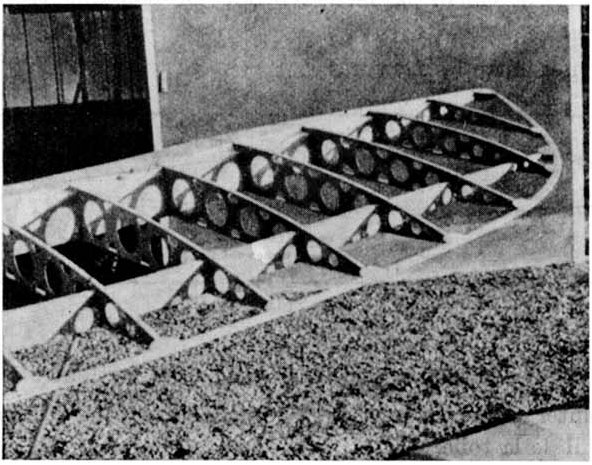
\includegraphics[width=\linewidth]{fig-47.jpg}
  \caption{The finished wing structure}
  \label{fig:fortyseven}
\end{figure}

After it dries overnight, remove the string and smooth, shape, and
polish the outline with the file.

\sectline

The fuel and oil tanks are placed in the forward wing, between the
center two ribs, a 15L one in front of the spar and a 20L one behind.
This gives a total flying time of about 5 hours and a range of 500km,
barring wind.

The tanks are placed on 3mm plywood floors \circled{245}, glued and
screwed under the center ribs, spar, and leading edge.  They are then
blocked into place and covered over.

The front and rear wings weigh 15 and 10 kilograms, respectively.

This is the moment to photograph them, because I hope you will not see
them thus again for a long time.  The photo is a good memory, and you
are welcome to send them to the author as a testimony of our
friendship --- he will be delighted!

\subsection{Covering}

The fabric is usually sold 1 meter wide.  For the forward wing, we
will use a sewing machine to join 6 strips, 3m 20cm long, at their
edges.

Wrap the wing chord, leaving the free edges at the trailing edge of
the wing \textit{(fig. \ref{fig:fortyeight})}.

\begin{figure}
  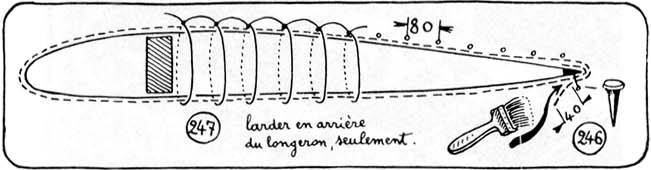
\includegraphics[width=\linewidth]{fig-48.jpg}
  \caption{Covering the wing}
  \label{fig:fortyeight}
\end{figure}

\begin{samepage}
Fully tighten the belly side by tacking the edge of the cloth around
the trailing edge:

\enumerate{
\item{Tack the cloth between the ribs \textit{1}.}
\item{Tack to rib \textit{6}, stretching between \textit{1} and
  \textit{6}.}
\item{Tack (about every 40mm) between 1 and 6, straight along the
  weave of the fabric.}
\item{Tack with four nails at both wingtips, stretching very tightly.}
\item{Tack between the wingtips and the ribs \textit{6}, stretching
  very tightly along the wingspan.}
\item{Stretch the belly cloth tight by pulling from the leading edge, and tack with one nail at each rib nose.}
\item{Flip the wing and tack the top surface (free edge folded and tacked on the belly side as shown at \circled{246}), pulling with all your might, and following the same pattern as for the belly.  Use tweezers to avoid bending your nails\ldots}}

\end{samepage}

Finish with the rounded part of the leading edge.

Nailing is more easily done with the wing upright on its leading edge
--- sweep the floor well so nothing injures the plywood!  A
helper\footnote{Or a stand --- Translator} holds it upright and
simultaneously holds the nailbox for you.  Climb on a 200mm stepstool
and stand on the opposite side from the nailing\footnote{Maybe
  M. Mignet means, \textit{get right across from your work}, as
  suggested by the Air League. --- Translator}.

Do your covering in hot, \textit{dry} weather, or in a \textit{dry},
heated room.  In wet weather, if you try to stretch\ldots a ray of sun
touches the wing, and you must begin afresh!  Cut away the excess
cloth, leaving a margin of 40mm after nailing.

Since our wing is now bagged like a mattress, let's stitch it up like
one.  Stitch \circled{247} along each rib with good hemp string
(Bessoneau N\textsuperscript{o} 8), and a mattress needle 22cm long
(Bazar H\^otel-de-Ville), knotting the string on the top of the wing
every 80mm, but not cutting the string between the knots.  Tighten
well as you go.  Thanks to the dihedral of the wing, these stitches
tighten the fabric very much.

All around the tips and trailing edges, the 40mm margin must be glued
with cellulose varnish, wetting the fabric above and below.  Let dry
completely (5 or 6 hours).

\subsection{Varnishing}

Choose a warm, dry, sunny day.  Work outside, in the shade, in the
afternoon.  Put the 20L can of cellulose acetate on a char.  Fill a
small pot of this varnish, and loading the 60mm fishtail brush, apply
the coating by wetting the canvas so it becomes translucent.  Spread
the excess around with additional brush strokes.

Don't economize on varnish; it's not there to look pretty, but to give
the fabric body.

Proceed gradually front to back, rib by rib.  Before moving on to the
next strip, smooth out any runs that have formed, but don't worry
about it too much.

In wet weather, the layers grow milky from condensation.  Try not to
work in such weather.

If it is warm, you can start the next coat two hours after the last
brushstroke.  Three coats is enough; an additional layer on top is
better.  After the first coat, lightly polish the entire surface with
fine sandpaper --- very effective.

Seams, gluings, and stitches must be covered with pinked tapes.  The
area is wet with varnish, then the tape, which is brushed into place,
soaked with varnish.  While it is drying, make sure the pinked edges
do not curl up.  Smooth them by rubbing with a cloth.  Before the
brush dries, wash it with soap and water.  The varnish will come off
in little white bits.

In the previous edition, there was a question of a little skylight to
see through the wing above you.  Don't bother with it.

\section{Rudder}

The rudder is of monospar construction
\textit{(fig. \ref{fig:fortynine})}.

\begin{figure}
  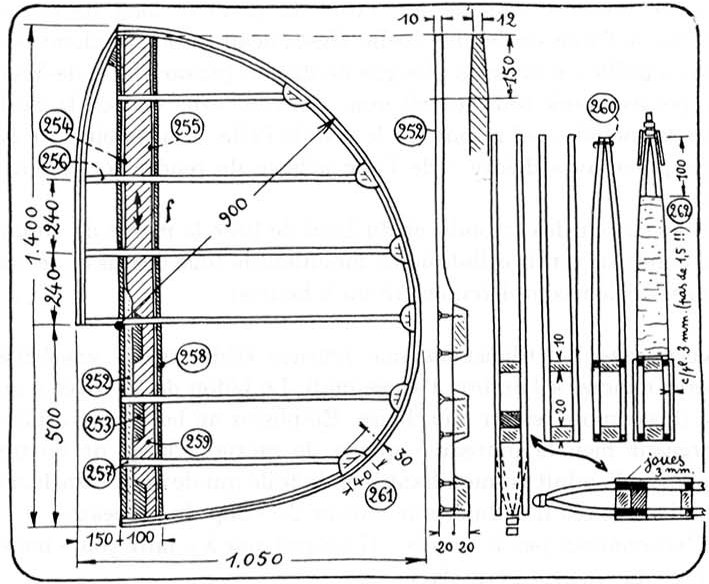
\includegraphics[width=\linewidth]{fig-49.jpg}
  \caption{The rudder}
  \label{fig:fortynine}
\end{figure}

A 20$\times$20 stick \circled{252} with hardwood reinforcements
\circled{253} is thinned as at \circled{254} to 20$\times$12.  It and
a 20$\times$10 slat \circled{255} form the spar caps.  Each 200mm,
nail on the 6$\times$12 strips that form the ribs.  The upper ones
extend beyond \circled{256} the spar, forming the leading edge and
acting as a slight aerodynamic balance.  The lower ones \circled{257}
end with the spar.  Place between the ribs 6$\times$8 strips
\circled{258} along each spar cap on both sides, and cover with a
strip of 3mm plywood \circled{259} 100mm wide and 1400mm long, with
the grain along its length.  This strip extends beyond the two narrow
ends of the caps, 12mm.  In the channel thus formed run two strips of
wood chosen for their straight grain, soaked for 10 minutes and bent,
then bound with plenty of glue after being nailed to the rib ends as
in \circled{260}.  Just like the trailing edge of the wings, the edge
is secured to the rib tails with gussets \circled{261}.

A 1.5mm plywood web \circled{262} stiffens each rib.

Cover the rudder just like the wings and apply 4 coats of varnish.

Time: rudder 4 hours, covering 1 hour; weight: 2kg.

\sectline

Now is the time to paint a beautiful emblem on the rudder.  It is the
signature of the amateur, and displays the craftsman's taste and
originality.

A good emblem is like lipstick on a pretty woman --- it completes the
\textit{toilette}; it is the stamp of seduction.

\sectline

The airframe is finished.  What remains is the fitting of the engine,
without which, like a face without eyes or a body without a soul, it
would be good for nothing.

\begin{figure}
  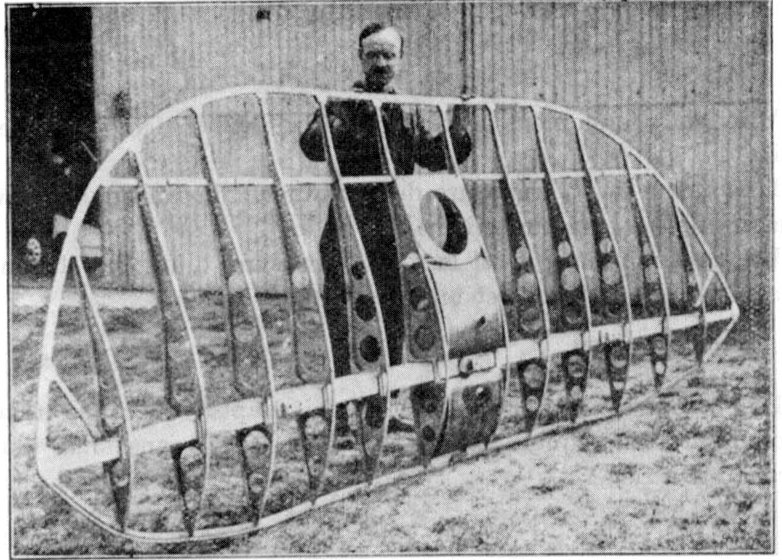
\includegraphics[width=\linewidth]{fig-50.jpg}
  \caption{M. Mignet with a wing of the old style, 4m in span.  The
    rear wing is identical except for the fuel tanks and the little
    window.  This wing has ribs in the old unsafe airfoil, and is
    shown to illustrate the overall wing assembly.}
  \label{fig:fifty}
\end{figure}


\chapter{The Engine}

Whether used for war, tourism, or sport, a suitable engine is the
essential basis of any aviation, no matter how aerodynamically sound
the aircraft is, even if it is a training glider.

Bad engine: failure.  Good engine: success.

\sectline

The foundation of my aeronautical exploits on the HM.8 was the motorcycle engine, unbolted from its frame and mounted on the fuselage to drive the propeller via reduction drive.  My amateur proceedings could supply nothing better.

It is possible that we may come back later in our 100\% amateur
proceedings with additional advice --- but for now, let's move on.

\sectline

At the time my flights were mere cricket hops --- barely 5 years ago
--- I begged a motorcycle manufacturer to assemble a 500cc
two-cylinder opposed engine on the same crankcase as his mass-produced
motorcycles, which were proven to be excellent.  This engine would
have provided 25hp at 40kg for 3000 francs.  I was asked to contribute
half the expenses, which rose to 12000 francs.  If I could have agreed
to pay half, this engine would have won the laurel in all Light
Aviation records.  Popular aviation would be four years ahead.  Who
knows where we might be today!!  I know it.  we would be today where
we will be in 4 years, perhaps not in France, but abroad where the
Light Aviation movement is a redoubtable force.  And all that lost by
hesitation, by smallness of mind, by laggardliness.

I did not have 6000 francs to spend, and the manufacturer decided to
pursue a different project, a 4-cylinder \textit{monobloc} engine for
light aircraft, of their own design, as mine were too rustic\ldots an
marvel of mechanics which could barely produce half the intended power
and almost bankrupted the company.

Planting to harvest\ldots be patient\ldots I stuck to it.

I next had the pleasure of meeting Ren\'e Poinsard, to whom I related
the basic ideas of my article on engines from \textit{Les Ailes}
n\textsuperscript{o} 511, April 2, 1931; in it I had called for a
1000cc flat twin of 25hp, with staggered cylinders, lubrication by
circulating oil, etc\ldots I'm not saying I created the
Poinsard-Mengin engine, but I do congratulate its author on having
chosen a formula well-proven elsewhere and turned to our purpose.
Instead of being drawn on by the craze for novelty, he relied on sane
judgment, and can thereby rely on years of experience.

\sectline

My old two-stroke was wind-broken, and a single-cylinder four-stroke
couldn't produce more power; I left for the \textit{Salon de la
  Motocyclette} (October 1932), having stuffed my briefcase with the
details of the HM.8, well illustrated with photos.  It didn't take me
long to find the Aubier Dunne booth with the 500cc two-cylinder
two-stroke, well-known to my amateurs, in front.  We quickly came to
an understanding, and a few days later, the Bois de Bouleaux heard
their engine humming.  They came out to my field often to test and
tweak the engine.  There were problems, they plied the wrench and
file, and finally the goal was achieved.  The engine ran well and
could produce 20hp indefinitely.

For three years, I was able to fly thanks to Aubier and Dunne.

When called by the big English paper, the Daily Express, to
demonstrate the Pou-du-Ciel to the British, I was preparing to cross
the English Channel, I had a failure of the four-stroke engine I was
using.  I didn't hesitate, in my embarrassment, but went straight to
Aubier and Dunne, and left without a worry to cross the Channel, even
though the engine was factory new. --- Overconfidence? --- No. ---
Confidence born of experience, in an engine I knew to be faultless.

\sectline

Other engines came along as the ``Pou fever'' spread, and the amateur,
having completed his machine, was at the point of mounting the engine.
I was deluged with questioning letters: Which engine should I choose?
What do you think of \textit{this} engine? --- I was just getting to
work on these novelties myself.

These new arrivals made me as welcome now as I had been ill-received
when I was making my first cricket-hops.  I must take this opportunity
to thank these manufacturers for their courtesy and their broadness of
vision.  With no view toward competition, they placed themselves at my
disposal in a spirit of frank collaboration.  Because of this, I was
able to answer the amateurs' queries with certainty, having flown
behind the main engines myself.

Shall I here compare their faults and virtues?

This afternoon, I flew a long time with first one, then another, and
then a third.  I have 4 Poux-du-Ciel in my laboratory, ready to go,
fitted with different engines.  This one has a bit of trouble taking
off, but is excellent at cruise, and burns but little fuel.  This
other consumes more fuel, but doesn't vibrate at all.  This last makes
less noise and climbs like crazy.  Which is the best?

Why does one man buy a Citro\"en, another a Peugeot, and another a
Renault?  Which car is best?  Who is right?

There are enough customers for all these engines to go around.  Each
company has a right to its time in the spotlight, and they will get it
if they produce merchandise of the quality the public expects and that
their advertising promises.

Therefore, I cannot say that one engine is better than another one.
They are \textit{different}, is the essential point, and they meet
different requirements.

\sectline

All that being said, light aviation has gained, thanks to the
Pou-du-Ciel, suitable engines.  That essential point achieved, the
rest is patience, perseverance, and planning on the part of the
amateur, and goodwill on the part of the government.

\sectline

\section{Some good engines:}

\textit{(M. Mignet begins by discussing some fine engines whose
  relevance is limited to his time.  I have included some of the
  illustrations, for the assistance they may provide in devising
  engine mounts for currently-viable engines.)}

\begin{figure}
  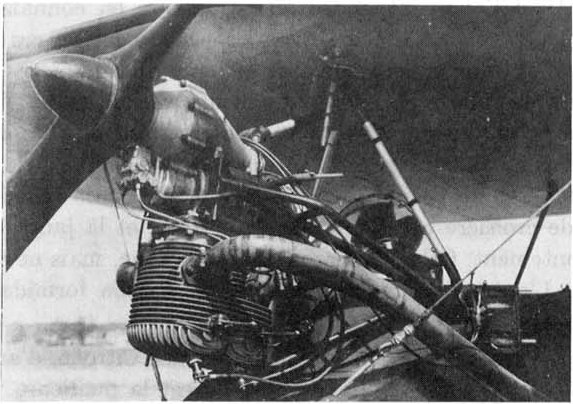
\includegraphics[width=\linewidth]{fig-51.jpg}
  \caption{The 540cc \textit{Aubier et Dunne} ``Channel'' model}
  \label{fig:fiftyone}
\end{figure}

\begin{figure}
  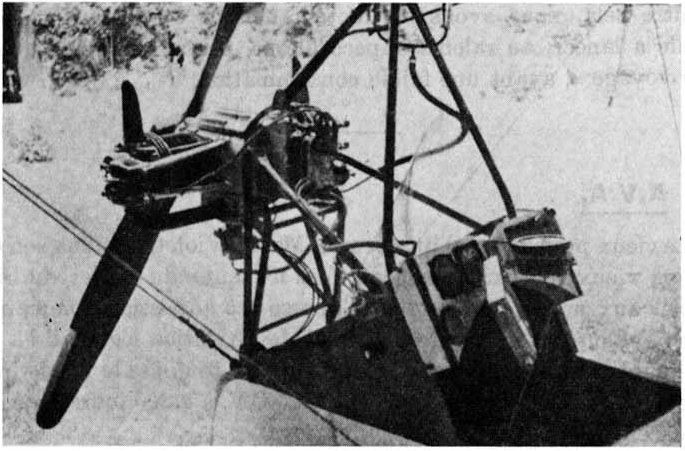
\includegraphics[width=\linewidth]{fig-52.jpg}
  \caption{The 25hp Poinsard-Mengin}
  \label{fig:fiftytwo}
\end{figure}

\begin{figure}
  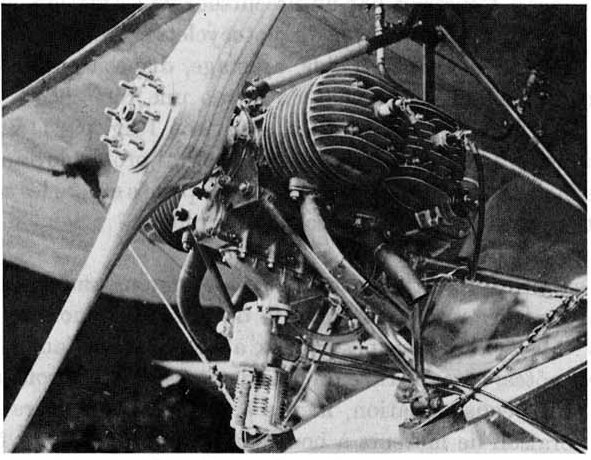
\includegraphics[width=\linewidth]{fig-53.jpg}
  \caption{The 25hp AVA engine}
  \label{fig:fiftythree}
\end{figure}

So, we must choose an engine.  A fight is brewing between 2- and
4-strokes.

The two-stroke has in its favor its extreme simplicity, as long as it
remains comparable to a motorcycle engine and is not loaded down with
too many accessories.  It has but one main defect --- its poor idle
--- and it has the advantage, for the amateur, of being very
affordable.

I wish all these engines would have one thing in common: that they
would turn the same direction, and have the same propeller hub!
\textit{Na\"if} that I am!  Do you think manufacturers past and future
want their engines to be compared in power using the same propeller?
Still, we are fortunate there are only two directions a propeller can
rotate; if there were seven, we would have seven engines rotating
different ways!  Apparently paying customers are entitled neither to
idle comparisons nor technical discussions\ldots

Finally, I would insist on the following points:

An engine must:

\enumerate{
  \item{not vibrate in flight --- essential for comfort and safety}
  \item{stay clean --- big selling point!}
  \item{feed from tanks placed at the height of the propeller axis}
  \item{have carb heat, to counter icing in winter}
  \item{have exhaust ports as low as possible}
  \item{have its mounting plate free of accessories}
  \item{have a variable or automatic ignition advance, or a magneto,
    to allow a safe departure; or have a starter, allowing even the
    weakest woman access to what will become her favorite sport: Light
    Aviation.}}

\section{Power}

As regards the Pou-du-Ciel, 25hp appears to be plenty of power.  At
cruise, the Pou is happy with 14 or 15hp; ten horsepower more ensures
a satisfactory takeoff and a service ceiling around 2000-2500 meters.

A more powerful engine (for the beginner) is worse than useless; it's
dangerous.  If the aircraft is badly balanced, it will still fly and
climb, but when the pilot cuts power, he risks finding himself in an
unrecoverable situation.

\sectline

We need not a powerful engine, but a \textit{faultless} engine.  The
one who shouts into every wind, ``Engines!  Compressors!'' may be
right when he addresses the sellers of flying gunships, but in private
aviation, popular aviation, safe aviation, this poor inexperienced
fool is talking nonsense.

The 1936 Pou-du-Ciel demands a \textit{continuous} 20-25hp, not 35
rabbits.  This engine should provide its power between 1500 and 2500
rpm, weigh 30 kilos, and cost 3000 francs.

Why do you hesitate, manufacturer?  You know nothing of aviation.  If
there were no engines, there could be no motorcycles; likewise, there
are no small airplanes because there are no engines.

Do the math, and you'll see that in four years you will have sold
forty thousand engines\ldots Are you decided?  Or does it give you a
tummyache?

May the good Lord bless you, or the Devil take you\ldots so be it!

\sectline

\section{Thermodynamics}

A few words about fuel would not come amiss.

Ignition of an explosive mixture quadruples its starting pressure.
The initial compression of 4kg/cm\textsuperscript{2} produces when
ignited a pressure of $4\times4 = 16$kg/cm\textsuperscript{2}.

8kg/cm\textsuperscript{2} produces 32; 16, 64; and so on, if it were
possible.

A motor produces more power as it rotates faster and its compression
ratio increases.  But\ldots there is a limit.

Very soon the mechanical elements can no longer obey.  Friction
absorbs any increase in power.

Too much compression, and the fuel-air mix \textit{detonates} before
the desired moment, producing a violent force that would break the
strongest engine.

Therefore, when we raise the compression ratio, we must provide the
engine with a specially-formulated mixture to ignite as late as
possible.  It's a problem of chemistry.

The normal mixture of air and gasoline detonates at a compression of 4
or 5.

Alcohol very effectively prevents detonation; it is therefore a
question of mixing it with gasoline.  But alcohol attracts water, and
water is the enemy of gasoline!  Such a mix becomes possible if the
water content of the alcohol is minimized and a binder added to
overcome the effects of the last traces of moisture.  Such binders
include benzol, ether, and butyl- and amyl- alcohols, among others.

An example proportion: 80\% gasoline, 10\% alcohol, 5\% benzol, 5\%
oil.

The proportion of alcohol may even exceed 25\%.  Benzol can also
replace alcohol.  There are even some mixtures that contain no
gasoline at all --- 100\% patriotic fuel!  With olive oil, alcohol,
and other locally-produced ingredients, we will no longer be dependent
on foreigners.

But that's another story entirely, and the owners of oil wells don't
want to think of nationalism with regard to our engine power\ldots!

Heavyweight motor oil works wonders for a high-compression engine.  Don't disdain them.

Finally, there are anti-knock products on the market that you can add
to your gasoline in a certain proportion.

\subsection{Drawbacks}

In cold, wet weather, mixtures of gasoline and alcohol tend to
separate.  The heavier alcohol settles to the bottom.  If there is oil
mixed with the fuel, the oil floats on top of the gasoline, and the
engine, running on pure alcohol, is no longer lubricated --- it will
seize up forthwith.

\subsection{Anti-detonation coefficient} %% TODO: figure out if this
                                         %% is the best interpretation

Two liquids with opposite qualities go into these mixtures: heptane,
which promotes detonation, and octane, which prevents it.  This
mixture ignites at a known compression, for a specific mixture: for
example, 20\% heptane and 80\% octane.  The mixture is called 80
octane.  Any other mixture, of gasoline, benzol, alcohol, or whatever
else, of a proportion which ignites at the same compression, is
likewise called 80 octane.  This is a comparison index.

For example, ignition at compression of 4 indicates 69 octane; at 5,
72; at 6, 75; etc.

A lot of people talk about octane numbers without understanding what
they're saying, and mechanics don't understand it either.  Beware the
octane ratings you see advertised.

Just like in photography, a good practice is to use the fuel and oil
recommended by the engine's manufacturer, and to not depart from it.

Avoid custom blends, untried innovations, and above all, the advice of
your friends.  When in doubt, ask the manufacturer.

Gasoline is to an engine as mushrooms are to a man: one is life,
another death.  Remember that everyone is selling something.

Be certain not to confuse

\begin{center}\textbf{detonation and preignition:}\end{center}

\begin{description}
\item[Detonation:]{

  The fuel mixture ignites explosively, all at once, at a certain
  compression.  The engine clicks.

  The sound of detonation is like a steel ball bouncing off of ice.
  It is dry and pungent, and very distinctive.  A detonating engine is
  about to stop running --- it is about to fail.  Reduce power to cool
  it, or look for some alfalfa for your wheels!
}
\item[Preignition:]{
  
  The fuel mixture ignites, aided by the heat of compression, but in
  contact with a part of the combustion chamber that is too hot: a hot
  particle of carbon or lead, a red-hot spark-plug tip, the
  poorly-cooled surface of a piston.  The engine knocks.
  Auto-ignition is less brutal than detonation, which overheats and
  shocks the engine more than anything, but it can cause the engine to
  quit without even a bump.  It gives the impression of a seized
  piston.}

\end{description}

This brings us to spark plugs; fast-turning, high-compression engines
are sensitive to spark plugs.  They need ``cold'' plugs, whose very
close electrodes are heavy and diffuse their heat to the outside or to
the mass of the plug by their good heat conductivity.  The magneto
permits easy starting despite these spark plugs.  Keep to the type of
spark-plug the manufacturer recommends --- \textit{this is an absolute
  law.}

\subsection{Carb jet}

The carb jet must be larger in proportion to the weight of the fuel;
here is an example for some particular engine:

\noindent\begin{tabular}{@{}p{5.5cm}@{\hspace{0.2cm}}p{1.8cm}@{\hspace{0.2cm}}p{1.8cm}@{}}
\hfill\bfseries Benzol& jet& 140 \\
\hfill\bfseries Normal gas& ---& 180 \\
\hfill\bfseries Heavyweight gas (25\% alcohol)& ---& 240 \\
\hfill\bfseries Pure alcohol (en course)& ---& 300 \\
\end{tabular}

\begin{figure}
  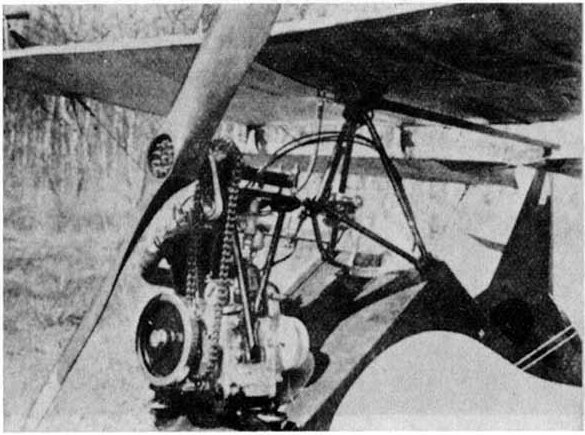
\includegraphics[width=\linewidth]{fig-54.jpg}
  \caption{The standard 500cc Chaise.  It flew 50 hours in Rul's HM.8.}
  \label{fig:fiftyfour}
\end{figure}

\section{Purchasing an engine}

When I advise you to buy a new engine, I'm assuming that you have the
necessary 4000 francs.  Perhaps that money will show up one day, if
you consider your hobby worth it, or if some outside investor is
impressed enough to allow you this purchase.

Maybe before you neither wanted to nor were able to risk so much on a
mere hobby.

You may have preferred to buy an engine second-hand and toss it out
later, replacing it with a better-made one.

It is necessary to define our situation.

According to the letters I got about the HM.8, and my own
tribulations, it appears that all engines of good manufacture are
about equal, from 500cm\textsuperscript{3}.

Among the old two-cylinder V's, Harley and Indian are second-bests.
They cannot be inverted.  Harley is the most serious.

The more recent 500cc single-cylinder four-strokes are workable,
preferably without a reduction unit.  They give from 17 to 20hp at
about 4000-4500rpm.  Some examples: JAP, Sturmey (English), DS
(French).  They can be inverted, modifying the oil system as needed.

\begin{figure}
  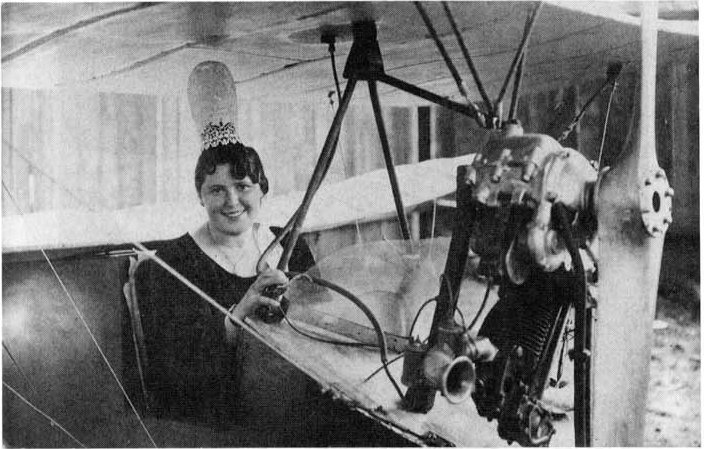
\includegraphics[width=\linewidth]{fig-55.jpg}
  \caption{Another inverted motorcycle engine... and its very
    good-looking pilot!}
  \label{fig:fiftyfive}
\end{figure}

Unless you find an exceptional opportunity of great quality, don't
spend more than 1500 francs.  There are, of course, opportunities; A
modified Harley costs 1000 francs; an Indian, 600.  They weigh 45kg
--- that's heavy.  Expect 12 kilos of accessories --- prop, reduction
gear, engine mount --- to complete the firewall forward installation.

I would despair at seeing you spend 3000 francs for a new non-aircraft
engine!

The used engine, a real bargain, will suffice to get you started.  The
worse it flies, the better pilot you will be come, but a trip around
the patch is the most you will be able to do --- if you make it.

\section{Mounting}

The inclined triangular platform of our fuselage makes it very easy to
install any sort of engine.

We will study two cases:

\begin{enumerate}
\item{

  You have purchased a light aviation engine, planned, suited, and
  perfectly tested, as was discussed above.

  No waiting, no studying, no risk.

  The manufacturer will supply an engine mount suited to and tested
  with the Pou-du-Ciel --- usually with my approval.}
\item{

  You have a used engine.

  Does this engine put out enough power to make the Pou-du-Ciel fly
  decently?

  Here are some data so you can figure it out right away.

  All you need to look at the number of revolutions per minute it will
  give with the propeller described in the next chapter.

  Test the propeller at a static point, in RPM.}
\end{enumerate}

\noindent\begin{tabular}{@{}p{1cm}@{\hspace{0.2cm}}p{6cm}@{}}
\bfseries 1350& Flight barely possible at high angles of attack.
Slow speed.  The engine will heat up and not hold up. \\
\bfseries 1400& Takeoff is difficult.  Must be light. \\
\bfseries 1450& Takeoff is easy.  At cruise it is possible to reduce the throttle a little.  Will the engine hold up? \\
\bfseries 1500& Good, but it could be better. \\
\bfseries 1550& It's a good start. \\
\bfseries 1600& Climbs at 2m/s.  Reaches 300m in 3 minutes\ldots cruises at \( \frac{1}{2} \) power.  Life is good!  Humanity swarms beneath your wheels. \\
\end{tabular}

\sectline

That being said, and to test my data --- who knows?  maybe your engine
is amazing --- this is how to proceed:

The engine mount which is given here is a welding job.  A professional
can do it easily; make sure you prepare the pieces in advance.  If
welding is unavailable to you, replace the tubes with angle iron
3$\times$30mm, riveted, with fittings modified to suit.  Rivets may be
made of 6mm drawn rod.  It's a provincial second-best.

Strive to place your engine upside-down, ``inverted'', with the
thrustline \textit{parallel} to the top rear and aligned with the
centerline of the fuselage, turned neither to the left or to the
right.

Keep it as low to the inclined platform of the fuselage as its size
allows, taking care that the front face of its housing --- the conical
tip of the shaft --- is directly above the front point of the
fuselage, with the axis of the motor horizontal.

\begin{figure}
  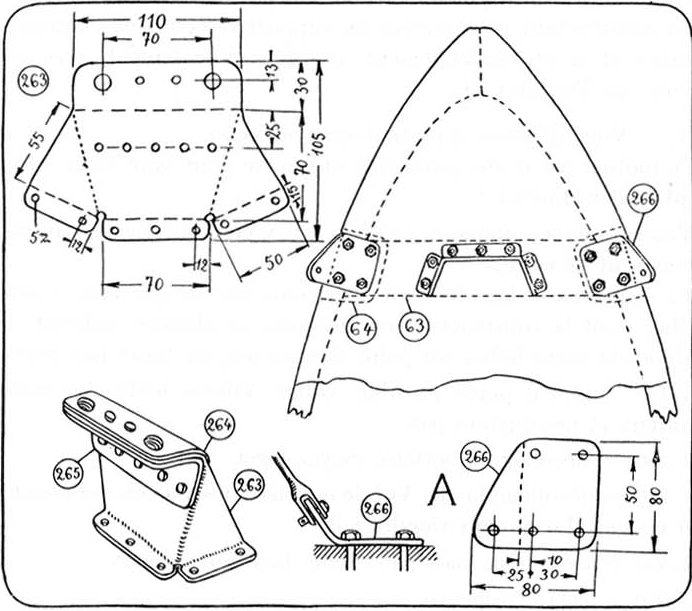
\includegraphics[width=\linewidth]{fig-56.jpg}
  \caption{Engine mounting details}
  \label{fig:fiftysix}
\end{figure}

The crankcase mounting flanges will be tightened by bolts (10mm
threaded rods in the case of the 540cc Aubier and Dunne, which we will
take here as an example) between the flanges \circled{267} made of 2mm
sheet metal (\textit {figures \ref{fig:fiftyseven},
  \ref{fig:fiftyeight}}). Ensure that the ears \circled{268} are
parallel.

\begin{figure}
  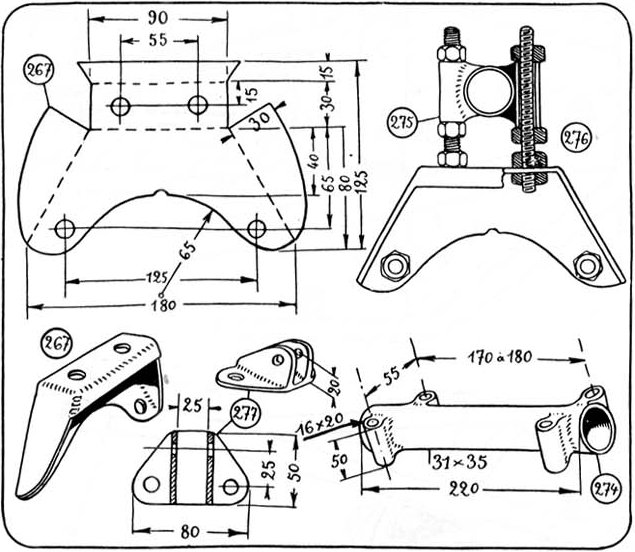
\includegraphics[width=\linewidth]{fig-57.jpg}
  \caption{Engine mount fittings}
  \label{fig:fiftyseven}
\end{figure}

Add to this a 16$\times$20 tube \circled{269} in such a way that,
welded to the two flanges, it falls into the fitting \circled{191} at
the feet of the cabane.  It will be good to heat this tube red and
bend it slightly, so that it meets the fitting squarely.  Fit the end
of this tube \circled{270} onto the front flange, trace the meeting
points, and take it to the welder.

\begin{figure}
  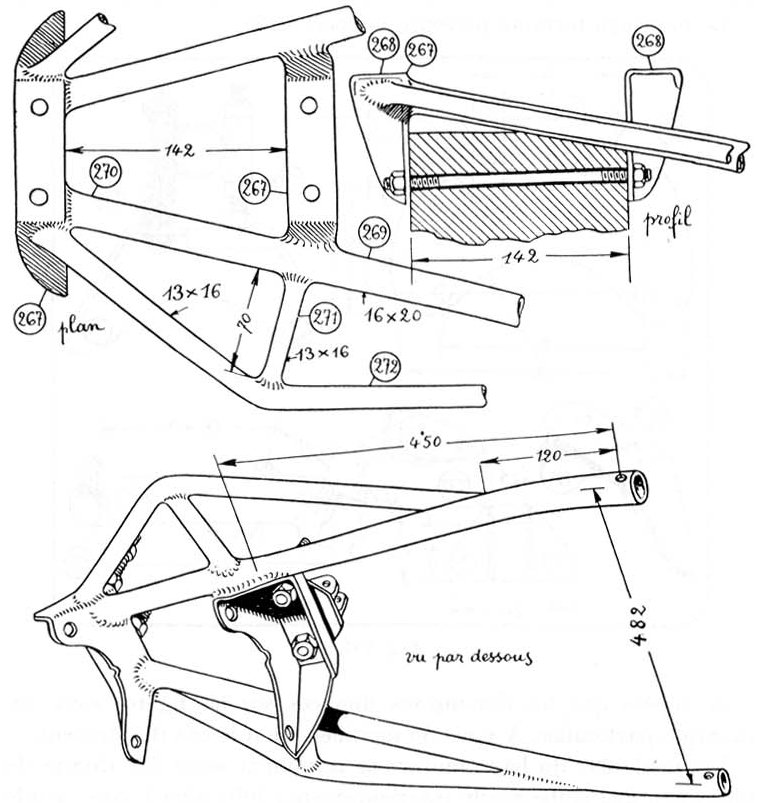
\includegraphics[width=\linewidth]{fig-58.jpg}
  \caption{Engine mount --- arrangement}
  \label{fig:fiftyeight}
\end{figure}

Bolt it back on the crankcase.

The welder will attach the tube to the second flange \textit{in
  place}.  Protect the engine with rags soaked in water, placing them
around the weld as soon as it is finished.

Remove the whole assembly and form a triangle with the spacer
\circled{271} and the tube \circled{272}, whose end is near to fitting
\circled{191} and will be welded last in place, 100mm from the
fitting.

The finished engine mount is shown at \circled{273}\footnote{Which
  does not appear, but refers to the lower drawing in Figure
  \ref{fig:fiftyeight}.}.

I repeat: the dimensions given in the figures are for one particular
example; it is up to you to modify them according to your case.

The feet \circled{297} of the engine mount are terminated according to
\circled{298} (filled with hardwood), \circled{299} (tube welded
internally), or \circled{300} (2mm tube welded externally).  The
latter way is best.  They are fastened in the brackets \circled{191}
of the cabane legs by a 7mm bolt.

This assembly is intended to control the engine's side-to-side
oscillation.

The engine will be supported on the other hand by two 16$\times$20
tubes welded or bolted on each side, somewhere on the crankcase or on
the flanges \circled{267}, with their feet welded on the wing bracing
fitting \circled{266} on the inclined platform.  That way, the engine
is secure, completely triangulated.

If, when running, you see the cylinder heads vibrate laterally, use
their fastening bolts to attach them to the rods that are connected
rigidly to the fitting \circled{266}.

The piece at \circled{263} is the old support for the 540cc Aubier and
Dunne, inverted and fastened to the two rear breech bolts.
  
\end{document}
